 \documentclass[conference]{IEEEtran}
\usepackage{subfig}
\usepackage{wrapfig}
 \usepackage{amsmath}
 \usepackage{url}
 \usepackage{pifont}
 %\usepackage{times}
\usepackage{rotating}
%\usepackage{balance} 
\usepackage{color, colortbl}
\usepackage{graphicx}
\usepackage{algorithmicx}
\usepackage[running]{lineno}
\usepackage{program}
\usepackage{cite}
\usepackage{alltt}
\newcommand{\eq}[1]{Equation~\ref{eq:#1}}
\newcommand{\bi}{\begin{itemize}}
\newcommand{\ei}{\end{itemize}}
\newcommand{\be}{\begin{enumerate}}
\newcommand{\ee}{\end{enumerate}}
\newcommand{\tion}[1]{\textsection\ref{sec:#1}}
\newcommand{\fig}[1]{Figure~\ref{fig:#1}}
\definecolor{lightgray}{gray}{0.975}
\usepackage{fancyvrb}
\usepackage{stfloats}
\usepackage{multirow}
\usepackage{listings}
\usepackage{amsmath}  
\DeclareMathOperator*{\argmin}{arg\,min} 
\DeclareMathOperator*{\argmax}{arg\,max} 


\usepackage{color}
\newcommand{\colorrule}[1]{\begingroup\color{#1}\hrule\endgroup}

\definecolor{darkgreen}{rgb}{0,0.3,0}

\usepackage[table]{xcolor}
\definecolor{Gray}{rgb}{0.88,1,1}
\definecolor{Gray}{gray}{0.85}
\definecolor{Blue}{RGB}{0,29,193}
\newcommand{\G}{\cellcolor{green}}
\newcommand{\Y}{\cellcolor{yellow}}


\definecolor{MyDarkBlue}{rgb}{0,0.08,0.45} 
\newenvironment{changed}{\par\color{MyDarkBlue}}{\par}

\newcommand{\ADD}[1]{\textcolor{MyDarkBlue}{{\bf #1}}}
\newcommand{\addit}[1]{\begin{changed}\input{#1}\end{changed}}

\usepackage{color}
\usepackage{listings}
\usepackage{setspace}

\definecolor{Gray}{gray}{0.9}
\newcommand{\kw}[1]{\textit{#1}}
\newcommand{\quart}[4]{\begin{picture}(75,6)
  {\color{black}\put(#3,3){\circle*{2.5}}\put(#1,3){\line(1,0){#2}}}\end{picture}}
% New Commands

\definecolor{Code}{rgb}{0,0,0}
\definecolor{Decorators}{rgb}{0.5,0.5,0.5}
\definecolor{Numbers}{rgb}{0.5,0,0}
\definecolor{MatchingBrackets}{rgb}{0.25,0.5,0.5}
\definecolor{Keywords}{rgb}{0,0,1}
\definecolor{self}{rgb}{0,0,0}
\definecolor{Strings}{rgb}{0,0.63,0}
\definecolor{Comments}{rgb}{0,0.63,1}
\definecolor{Comments}{rgb}{0.5,0.5,0.5}
\definecolor{Backquotes}{rgb}{0,0,0}
\definecolor{Classname}{rgb}{0,0,0}
\definecolor{FunctionName}{rgb}{0,0,0}
\definecolor{Operators}{rgb}{0,0,0}
\definecolor{Background}{rgb}{1,1,1}

\lstnewenvironment{python}[1][]{
\lstset{
mathescape,
numbers=right,
numberstyle=\scriptsize,
stepnumber=1,
numbersep=0.5em,
xleftmargin=0em,
framextopmargin=2em,
framexbottommargin=2em,
showspaces=false,
showtabs=false,
showstringspaces=false,
tabsize=2,
% Basic
basicstyle=\ttfamily\scriptsize\setstretch{0.8},
backgroundcolor=\color{Background},
language=Python,
% Comments
commentstyle=\color{Comments}\slshape,
% Strings
stringstyle=\color{Strings},
morecomment=[s][\color{Strings}]{"""}{"""},
morecomment=[s][\color{Strings}]{'''}{'''},
% keywords
morekeywords={[1]import,from,class,def,for,while,if,is,in,elif,else,not,and,or,print,break,continue,return,True,False,None,access,as,,del,except,exec,finally,global,import,lambda,pass,print,raise,try,assert, dot, norm, zip, sorted},
keywordstyle={[1]\color{Code}\bfseries},
% additional keywords
morekeywords={[3]fastmap, Line,bPruning,clister,train,leafs,weightedFeatures, exemplar,nearestLine,dist,displace,geometry,splitAcross2Points,leaves,How,nearest,bPruning,Stats,divide,recurse,weight1,project, furthest, split, WHERE,clusterer, getContours, envied, fWeight, nearestContour, projection, mutate, HERE, knn},
keywordstyle={[3]\color{Keywords}\bfseries},
morekeywords={[2]@invari},
keywordstyle={[2]\color{Decorators}\slshape},
emph={self},
emphstyle={\color{self}\slshape},
firstnumber=last
%
}}{}
 
\title{Learning Actionable Analytics 
 (with applications for reducing defects and reducing runtimes)}
\author{
% You can go ahead and credit any number of authors here,
% e.g. one 'row of three' or two rows (consisting of one row of three
% and a second row of one, two or three).
%
% The command \alignauthor (no curly braces needed) should
% precede each author name, affiliation/snail-mail address and
% e-mail address. Additionally, tag each line of
% affiliation/address with \affaddr, and tag the
% e-mail address with \email.
%
% 1st. author
Rahul Krishna, Tim Menzies, Xipeng Shen\\
       \affaddr{Computer Science, NcState, USA}\\
       \{i.m.ralk, tim.menzies, xipengshen\}@gmail.com
% 3rd. author
 % use '\and' if you need 'another row' of author names
% 4th. author
\and
 Andrian Marcus\\
       \affaddr{Computer Science, UtDallas, USA}\\
       {amarcus@utdallas.edu} }


  \pagestyle{plain}
\begin{document}
  \maketitle
  
  % make the title area
  
   
  \begin{abstract}
 As business users demand more insightful
 analytics, data scientists need to change
 their tools. Instead of merely predicting 
 some result, they also need tools that generate ``plans'';
 i.e. specific suggestions on  how to change values in order to
 improve on some predicted value.
 
 This paper proposes one such planner. ``HOW'' is a 
 tool for proposing changes to independent
 variables in order to improve on 
 the predictions of the dependent variables. Unlike other approaches
 for learning optimizations to software, HOW does not require
 an underlying of the domain. Also, HOW's plans
 are designed to result in {\em minimal displacement}
 to current practice.
 
 This paper uses  HOW to learn methods
 to reduce defects and decrease program runtime.
 For the test data of this paper, the improvements generated by HERE can reduce
 defect counts as well as runtimes by up to
 50\% of their original values.
  \end{abstract}
  \begin{IEEEkeywords}
Defect prediction, configuration, prediction, planning, instance-based reasoning.
  \end{IEEEkeywords}
  
\section{Introduction}
Business  users   now demand   data mining tools
that  support a  business-level
interpretation of that data. For example,
at a  panel on software analytics at ICSE'12,
industrial practitioners lamented the state of the art in data mining
and software engineering~\cite{menzies12a}. Panelists commented that
``prediction is all well and good, but what about decision
making?''. That is, these panelists are more interested in the interpretations
and follow-up
that occurs {\em after} the mining, rather than just  the mining itself. For example:
\bi
\item 
Instead of just accepting  {\em predictions} on how many 
 software defects
to expect,  business users might now demand a {\em plan} to
reduce the likelihood of those defects;
\item Instead of just accepting {\em predictions} on the runtime
time of their software, business users might now demand
a {\em plan} to reduce that runtime.
\ei
In this paper, we say   a ``plan'' is a  set of changes
proposed  in order to better achieve some goal. 
Specifically, for every $Z$  that requests a plan $\delta$, we want
to adjust the attributes $Z_j$ as follows:
\begin{equation}\label{eq:one}
Z_j = Z_j + \delta_j
\end{equation}
The usual way such plans are generated in the SE literature
is via some search-based method. Recently, we have made  some progress
in this area with the  GALE optimizer~\cite{krall14}. 
Like other search-based algorithms,
 GALE executes by proposing multiple $\delta$s
 (one for each generation in an evolutionary program).
 In practice, GALE makes
 extensive changes to initial sample of project data
 (perhaps 
100s to 100,000s of mutations). Each of these mutations
is reassessed using some domain model.
GALE runs faster than standard search-based SE tools~\cite{deb00a,zit02} since
it explores  the principle components
 of the project data (rather than   the raw data). Since it explores
 a smaller space, it also
 terminates much faster than standard optimiser; e.g. for one large model, 4 minutes versus 7 hours~\cite{krall14}. 

When presented to some  users, the GALE approach was challenged by
two business users.   Note that the following issues
challenge not just GALE, but also  any  optimization algorithm  that makes
extensive use of mutation  and domain models such as
NSGA-II, NSGA-III, SPEA2, IBEA, particle swarm optimization, MOEA/D, etc.~\cite{deb00a,zit02,zit04,%
deb14,Cui2005a,zhang07:TEC}.


One  user asked:
\begin{quote}
ISSUE~\#1: {\em ``What if I only want the minimum useful change, not
the maximum possible?''}
\end{quote}
Note here that this business user is asking for solutions  that do not require extensive 
changes to their current  approaches. 

Later in that discussion, another business user asked:
\begin{quote}
ISSUE~\#2: {\em ``But what if I do not have a domain model of my business?''}
\end{quote}
This also is a legitimate issue.
Building and certifying a model  can  takes  long time, especially in software engineering. For  example, in previous work~\cite{me07f} we used models
developed by Boehm's group at the University of Southern California.
Some of those models took decades to develop and mature (from 1981~\cite{boehm81} to 2000~\cite{boehm00b}). 
Also, even when there is an existing model, they can require
constant  maintenance lest they become out-dated. Elsewhere, we have described our
extensions to the USC models to enable reasoning about agile software developments. 
It took many months to implement and certify those extensions~\cite{me09i,me09j}.
The problem of model maintenance is another
motivation to look for alternate methods that can be automatically updated whenever new data arrives.
Further, sometimes  it is easier to access instances of a model's behaviour than the model
itself. For example, in prior work with Martin  Feather from the Jet Propulsion 
Laboratory~\cite{fea02a},  our research partner could not share a
propriety model from within the NASA firewalls. However, they could share 
logs of the input/output of that model.


Every challenge is an opportunity to explore  a new approach.
If we  restrict $\delta$ to very small changes, then any 
predictive data miner applied to the original data could also be used
to assessed the mutated data (proviso: we have to guarantee that
the mutations do not leave the space of examples present in the original data).
Note that this approach addresses ISSUE~\#1 since it only uses minimal changes.
It also addresses  ISSUE~\#2 since, when lack a domain model, we automatically
create one (via data mining).

 
This paper presents HOW, a novel planner for learning actionable analytics via
minimal changes. 
In the experiments shown below, we see that HOW's plans  can significantly
reduce the  expected
value of:
\bi
\item The software defects found in  the object-oriented JAVA systems explored in 2010 by Jureczko et al.~\cite{jureczko10};
\item The runtime of the  software systems whose configurations
are explored in 2013 by Seigmund et al.~\cite{sven12};
\ei
This paper makes five contributions:
\be
\item The HOW  instance-based planner (which has not been presented before).
\item The experiments of this paper show that HOW planner is useful for real-world tasks;
e.g. reducing the
expected values of the Jureczko software defects and the Seigmund software runtimes.
\item Apart from HOW, we  also offers a general framework for using  predictive system to build planners;
\item Further, we offer a  test to recognizes  when we should {\em not}  plan: specifically,
planning is
not recommended in domains with  poorly performing predictors;
\item Last, we  offer a general verification rig for assessing the value of plans generated within this rig.
\ee 

\section{How to Build ``HOW''?}\label{sec:mm}

\subsection{Design}
A general model for {\em predictors} is as follows. 
During testing, each test instance gains a prediction 
by finding which region of the data it falls into.
During training, those regions are inferred from
divisions that ``chunk'' together regions with instances
with similar properties. These dividers can be categorical (as in the case of decision trees) or probabilistic (as in the
case of Naive Bayes) or learned via some distance minimization
process 
(as in the case of support vector machines) or generated
directly by some clustering algorithm. 


\begin{figure}[t!]
\small
~\hrule~

{\bf \fig{where}a: top down clustering:}

Data can be rapidly and recursively divided   as follows.
Find   two   distance instances,  $X,Y$
by picking any instance $W$ at random, then setting $X$ to its most
distant instance, then setting $Y$ to the instance most distant from
$X$~\cite{fastmap}
(this requires only $O(2N)$ comparisons
of $N$ instances).
Next, project each instance $Z$
onto a line that  runs between $X,Y$ using the cosine
rule of \fig{where}b. After that,  split the data at the median $x$ value of all instances and
recurses on each half  (stopping when
one half has less  than $\sqrt{N}$ of the original population). For more details. \fig{howcode}, line~76, 

~\hrule~
 
{\bf \fig{where}b: finding distances:}

In the \fig{where}a, to compute distances, we use
the Euclidean measure recommended for
instance-based reasoning by Aha et al.~\cite{aha91};
i.e. $\sqrt{\sum_iw_i(X_i-Y_i)^2}$ where $X_i,Y_i$
where values are  normalized 0..1 for the range min..max and 
$w_i$ is some importance weight given to attribute $i$.
Usually, $w_i=1$ but it can be adjusted using, say,
the feature weighting methods of \fig{where}d. 
 
 ~\hrule~
 
{\bf \fig{where}c: 3 point geometry:}
 
Let   $X,Y$ be two points joined by  a line  length $c$.
A third point, $Z$, has distances  $a=dist(Z,X)$ and
$b=dist(Z,Y)$ to $X,Y$, respectively.
According to the cosine rule,   $Z$ projects onto  $\overline{XY}$
at distance $x=(a^2 + c^2 - b^2)/(2c)$ from $X$.
Further, according to Pythagoras' theorem, $Z$ stands at a distance
$y = \sqrt{a^2 - x^2}$ from the line $\overline{XY}$. For more details, see  \fig{howcode}, line~59.

~\hrule~

{\bf \fig{where}d: feature weighting:}

HERE's feature weighting algorithm
comes from the CART regression tree learner~\cite{Breiman1984}.
It sorts independent variables
 according to how well they can reduce the variability
of a  numeric objective.
If we split some column $i$ of independent numeric data  into $N=n_1 + n_2 + ..$ splits,
then the expected
value of the objective value of the split  is $w_i = \sum_i v_in_i/N$
where $v$ is the standard deviation of the objective.
A recursive procedure can  find those divisions $n_1,n_2,...$ by (a)~sorting a numeric column,
then split at $\argmin_i w_i$, then recursing into each half.  For more details, see  \fig{howcode}, line~109.

~\hrule~
 
\caption{Sub-routines within HOW.}\label{fig:where}
\end{figure}



\begin{figure} 
\begin{python}[right]
def HERE(trainingData, testingData):
  training(trainingData)
  return [nearest(z).displace(z) 
          for z in testing]

def training(trainingData):
  Line.using = what2Use(trainingData)
  clusters = cluster(trainingData):
  for cluster in clusters:
    one = examplar(cluster)
    two = examplar(nearest(one, clusters))
    Line(one,two)
  
def what2Use(trainingData):
  second  = lambda lst: lst[1]
  weights = map(second,
                sorted(featureWeighting(trainingData)))
  use    = int(len(weights)*Line.B)
  return [i for i,_ in enumerate(weights[:use])]

def nearestLine(z):
  out,least=None,10000
  for line in Line.all:
    d = line.dist(z)
    if d < least: out,least = line,d
  return out
\end{python}
\caption{Instance-based Planning using HERE.
Testing data is {\em displaced}
towards   the $X$ point of the nearest {\tt Line} (defined in \fig{line})
The {\tt geometry} method comes from \fig{code1c}.
The {\tt featureWeighting} function comes from \fig{code1a}.
The {\tt cluster} function comes from \fig{fastmapCode}.
}\label{fig:HERE}   
\end{figure}



\begin{figure} 
\begin{python}[right]
class Line:
  "Lines connect a worse cluster Y to a better one X"
  all   = []
  using = []
  F     = 0.5
  B     = 0.5
   def __init__(i,x,y):
    if x.score < y.score:
      x,y = y,x
    i.c = dist(x,y) 
    i.obj = len(x) 
    Line.all += [i]
  def displace(i,z):
    for j,(xj,zj) in enumerate(zip(x,z)):
      if not j == i.obj and  j in Line.using:
         z[j] = zj + Line.F*( xj. - zj
    return z
  def dist(i,z):
    _,out = geometry(i.x,i.y,z)
    return out
  def exemplar(i,cluster):
    #Apply the rules at end of section II.B
\end{python}
\caption{The primary data structure of HOW
is the {\tt Line}.
Training data is converted into a set of {\tt Line}s,
each of which is defined by a $X,Y$ pair, where $X$
has better scores than $Y$. }\label{fig:line}
\end{figure}




\begin{figure} 
\begin{python}[left]
def dist(x,y):
   "See Aha et al. reference [22]. XXX"
   
def geometry(x, y, c, z): 
  a = dist(z,x)
  b = dist(z,y) 
  x= $(a^2 + c^2 - b^2)/(2ac)$ 
  y=  $\sqrt{a^2 - max(x,0)^2)}$
  return x,y
  
def nearest(x,data):
  return furthest(x,data,best=1000,better=lt)
 
def furthest(x,data, best= -1, better=gt):  
  out = None
  for one in data:
    d = dist(one,x)
    if gt(d,best): out, best = y, d
  return out
\end{python}
\caption{Some routines for 3 point geometry,  from \fig{where}.c.}\label{fig:code1c}
\end{figure} 


\begin{figure}
\begin{python}[left]
def featureWeighting(cols):
   obj = len(cols[0])
   return sorted(weight1(col,i,obj) 
                for i,col in enumerate(cols)
                if not i == obj)

def weight1(i,obj,col):
  pairs = sorted([row[i],row[obj] for row in col])
  n     = length(col)
  return sum(v*n1/n for v,n1 in recurse(pairs,[])),i

def recurse(this,cuts):
  cut,sd = divide(this)
  if cut:
    recurse(this[:cut],cuts)
    recurse(this[cut:],cuts)
  else:
    cuts += [(sd,len(this)]
  return cuts
    
def divide(this,tiny=2):
  lhs, rhs = Stats(), Stats(x[1] for x in this)
  n, least, cut = rhs.n*1.0, rhs.sd(), None
  for j,x in enumerate(this):
     if lhs.n > tiny and rhs.n > tiny:
       tmp = lhs.n/n*lhs.sd() + rhs.n/n * rhs.sd()
       if tmp < least:
          cut,least = j,tmp
     rhs - x[1]
     lhs + x[1]
  return cut,least
  
class Stats():  
    def __init__(i,inits=[]):
      i.n = i.mu = i.m2 = 0.0
      map(i.__add__,inits)
    def sd(i) :  
      return (max(0.0,i.m2)/(i.n - 1))**0.5
    def __add__(i,x):
      i.n  += 1
      delta = x - i.mu
      i.mu += delta/(1.0*i.n)
      i.m2 += delta*(x - i.mu) 
    def __sub__(i,x):
      i.n  -= 1
      delta = x - i.mu
      i.mu -= delta/(1.0*i.n)
      i.m2 -= delta*(x - i.mu) 
\end{python}
\caption{Feature weighting, from \fig{where}.d.}\label{fig:code1a}
\end{figure}

\begin{figure} 
\begin{python}[left]
def cluster(data, n,lvl=100):
  if lvl < 1: 
     return data # stop if out of levels
  leafs = [] # Empty Set
  x,y,left,right = splitAcross2Points(data) 
  if len(left) > $\sqrt{n}$:  
     leafs += cluster(left, n, lvl - 1)  
  if len(right) > $\sqrt{n}$:  
     leafs += cluster(right,n,  lvl - 1) 
  data.has = dict(x=x,y=y,
                 l=left,r=right,
                 leafs=leafs)
  return leafs
  
def splitAcross2Points(data): 
  tmp = random.choose(data)
  x = furthest(tmp, data)
  y = furthest(x, data) 
  c = dist(x,y)  
  if x.scores < y.scores:
     x,y = y,x 
  for one in data.members: 
    one.pos = geometry(x,y,c,one)
  data = sorted(data) # sorted by 'pos.x'
  return x, y, split(data)
  
def split(data):   
  mid = len(data)/2; 
  return data[mid:], data[:mid]
\end{python}
\caption{Clustering. Lines 16,17,18 come from~\cite{fastmap}. }\label{fig:fastmapCode}   
\end{figure}




Those same regions can be used for instance-based 
{\em planning}-- but instead of leaving test instances in the regions
found during training, we {\em displace} them towards regions
with better objective scores.
To achieve this, 
during training, HOW clusters data using the procedure of \fig{where}a,
then draws {\tt Line}s between the centroids of  clusters $X,Y$ that are nearest
neighbors.
By convention, we say that the cluster containing $X$ has the  better objective scores. This means we can say that the {\tt Line} is a useful direction for displacing
data; i.e.  away from $Y$ and towards $X$ (for an implementation of such a {\tt Line} class, see \fig{howcode}, line~1).
 During testing,  HOW   finds the  nearest {\tt Line} to every test instance. That  test instance is   then displaced towards the better end
of that line; i.e. towards  $X$ (see \fig{howcode}, line 53).

An important design decision with HOW 
is how to determine the exact {\em direction} and {\em magnitude} of the
displacement.  Following on from the discussion around   ISSUE~\#1,
we note that a design goal of HOW is
{\em minimal displacements} of project data.
To implement minimal displacement:
\bi
\item
HOW sorts  the independent variables
using the procedure of  \fig{where}d. It then only
displaces the    best $B$\%  of that sort, while leaving the rest untouched
(see \fig{howcode}, line 38).
In  the experiments shown below,  we explore   $B \in \{25,50,100\}\%$.
\item
HOW also  limits displacement
to very small regions in the space of the training data (never more that the separation
of the two closest clusters).  HOW's clusterer divides  data into many   small clusters containing
$\sqrt{N}$ of the population (using the {\tt cluster} function, \fig{howcode}, line 76).
HOW   limits displacement to  \mbox{$0 \le F \le c$}, where
$c$ is the distance between the two closest clusters. 
In  the experiments shown below,  we explore
\mbox{$F\in \{0.25, 0.5, 0.75\}$}.
\ei
Turning now to the displacement {\em direction},
our experiments show that it useful to  carefully reflect on exactly where HOW should  push each test instance.
HOW replaces each cluster   with one {\em exemplar} that best
characterizes the data in that cluster. It then displaces the
test data towards that exemplar, as shown in \fig{howcode}, line 19. In summary, 
If  $Z_j$ is an independent variable within the
test instance $Z$ and  $X$ is the exemplar found at training time,
then we displace $Z$ as follows:
\[Z_j =  Z_j + F*(X_j - Z_j)\]
Here, $F$ is the  magnitude controller, discussed above. Note that this
this equations satisfies our definition of a ``plan'' as offered in
\eq{one} in the {\em Introduction}

The experiments of this work showed that different kinds of data require
different kinds of exemplars.
\bi
\item
For the Jureczko data, the objective score
is a boolean that is true if defects have been noted
for that class. 
For this kind of data with discrete objectives,
the data, 
has very little to  differentiate between the objective scores
so we just set the exemplar to  
an instance synthesized from the median values of the instances
in that cluster.
\item
For the Seigmund data,
the objective score is the runtime of the test suite of a compiled program.
For this kind of data with numeric objectives,
the exemplar  is the instance in a cluster
with  best objective score.
\ei 

  
  
\begin{figure}[!t]
\small 
\[
\begin{array}{r}
\mathrm{project}\\
\mathrm{data}
\end{array} 
\left\{\begin{array}{l}\mathit{train}
        \left\{\begin{array}{l}
                \mathrm{learn\;a\;}\mathrm{predictor\;}\mathrm{(e.g.\;via \;Random\;Forest)}\\
                \mathrm{learn\;a\;}\mathrm{planner\;}\mathrm{(e.g.\;via \; HOW)}
              \end{array}\right.
       \\
      ~\\
\mathit{test}  
    \left\{\begin{array}{l@{~}l}
           \mathit{before}& =\mathrm{predictor}(\mathit{test})\\
           \mathrm{\bf if\;}\mathit{before} & <  \mathit{satisfactory}\\
           \mathrm{\bf then}  & \mathrm{{\bf return}\; 0}\\~\\
           \mathrm{\bf else} &
           \left\{
            \begin{array}{l}
                \mathit{test'} = \mathrm{planner}(\mathit{test})\\
                \mathit{after} =\mathrm{predictor}(\mathit{test'})\\ 
                \mathrm{{\bf return}\;} \mathit{before},\mathit{after}
            \end{array}
          \right.
   \end{array}\right.
\end{array} \right. 
\]
 
\caption{How to use {\em predictors} for {\em planning}.}\label{fig:work}
\end{figure}



\subsection{Assessment}\label{sect:assess}
In the experiments shown below,  HOW comments  on how to reduce
software defects by adjusting certain static code parameters of the code\footnote{Such parameters can be manually adjusted by programmers or (for large scale changes) automatically adjusted using code refactoring
tools, as shown by Binkely et al. in 2006~\cite{Binkley2006} and more recently by Mkaouer et al. in 2015~\cite{Mkaouer15}.}. How are we to verify that HOW's recommendations actually work? 

Some organizations have the resources to 
run repeated trials to assess the effect of different treatments.
For example, in one remarkable recent study, Bente et al. report results
were the same specification was developed into a product by four different organizations~\cite{Anda2009}. Given those kind of resources, it would be possible
to (say) take a code base, assign it to $N$ different teams, apply
HOW's plans the code used by  $N/2$ teams, then check in 12 months time
if those halves of the teams have fewer defects than the other.  

Very few industrial or research groups have access
to the kinds of resources using by Bente et al. (evidence: in the size years since the
publication of that work, we know of only one of two similar studies). Hence, it
we wish to verify HOW's plans, then some other framework is required that is less
resource intensive.
 




We propose using prediction systems (built by data mining) as a verification
tool for planners. In domains with data, from which data miners can build
predictors of adequate performance, then those predictors can assess the value
of the changes proposed by HOW.

As shown in \fig{work}, our proposal divides
project data  into two disjoint sets {\em train} and {\em test}
(so \mbox{{\em train} $\cup$ {\em test} $=\;\emptyset$}).
Next, from the train set, we build both a {\em planner} as well
as a {  predictor}. Our general framework does not   commit to any particular  choice
of { planner} or { predictor} but, for the purposes of this paper, 
our { planner}
will be HOW  and our
our { predictors} will be the Random Forest and Random Forest
Regressor taken from the SciKit
Learn toolkit~\cite{Pedregosa2012}. The Random Forests procedure is explained in \fig{rr}. 

\begin{figure}[t!]
\small
\begin{tabular}{|p{.95\linewidth}|}\hline
 Decision tree learners find the attribute whose value's
select for for sections of the data with least variation in the class
variable. Decision tree learners then recurse on each selection~\cite{breiman84}. 

A random forest is a set of decision trees, each built
from some random subset of the rows and columns. The conclusions
of the forest are a ``vote'' generated by all the trees~\cite{Breiman2001}. 

A standard Random Forest predicts for a discrete class variable while
a Random Forest Regressor generates numeric predictions.\\\hline
\end{tabular}
\caption{Random Forests and Random Forest Regressors.}\label{fig:rr}
\end{figure}


Turning now to the {\em test} data, this is passed to the { predictor}
to generate a baseline {\em before} performance score.
Note that if our { predictors} fail to perform adequately on the test data,
then we cannot trust them to comment on our plans. Accordingly,
if that performance is unsatisfactory, we abort.
Else, we (1)~apply the { planner} to alter the {\em test} data;
then (2)~apply the { predictor} to the altered data {\em test'};
then (3)~return data on the {\em before,after} predictions.




\begin{figure*}[!t]
\scriptsize
   \begin{center}
   \begin{minipage}{.46\linewidth}
    \begin{tabular}{r@{~}|l@{~}|r@{~}|l@{~}|r@{~}|r@{~}|} \cline{2-6}
   & \multicolumn{5}{c|}{ }\\ 
   
   & \multicolumn{5}{c|}{ Data set  properties}\\ 
   & \multicolumn{5}{c|}{  }\\ 
           & \multicolumn{2}{c|}{training}   & \multicolumn{3}{c|}{testing}      \\ \cline{2-6}
   data set      & versions           & instances & versions     & instances    & \% defective             \\ \hline
        jedit    & 3.2, 4.0, 4.1, 4.2 & 1257      & 4.3          & 492          & 2 \\
        ivy      & 1.1, 1.4           & 352       & 2.0          & 352          & 11 \\
        camel    & 1.0, 1.2, 1.4      & 1819      & 1.6          & 965          & 19 \\
        ant      & 1.3, 1.4, 1.5, 1.6 & 947       & 1.7          & 745          & 22 \\
        synapse  & 1.0, 1.1           & 379       & 1.2          & 256          & 34 \\
        velocity & 1.4, 1.5           & 410       & 1.6          & 229          & 34 \\
        lucene   & 2.0, 2.2           & 442       & 2.4          & 340          & 59 \\
        poi      & 1.5, 2, 2.5        & 936       & 3.0          & 442          & 64 \\
        xerces   & 1.0, 1.2, 1.3      & 1055      & 1.4          & 588          & 74  \\ 
        log4j    & 1.0, 1.1           & 244       & 1.2          & 205          & 92   \\
        xalan    & 2.4, 2.5, 2.6      & 2411      & 2.7          & 909          & 99  \\\hline 
        
        
    \end{tabular}\end{minipage}\begin{minipage}{.4\linewidth}
    \begin{tabular}{|rrr|rrr|rr|l} \cline{1-8}
      \multicolumn{8}{|c|}{  }\\
      \multicolumn{8}{|c|}{  Results from learning}\\
       \multicolumn{8}{|c|}{   }\\
   \multicolumn{3}{|c|}{untuned} & \multicolumn{3}{c|}{tuned} & \multicolumn{2}{c|}{change}\\
  \cline{1-8}
  
  pd & pf & good? & pd & pf & good? & pd & pf\\\cline{1-8}
  50 & 27 &   & 64 & 28 & y & 14 & 1&$\star$\\
  65 & 35 & y & 65 & 25 & y & 0 & -10&$\star$\\
  50 & 30 &   & 62 & 41 &   & 12 & 11\\
  66 & 21 & y & 63 & 18 & y & -3 & -3\\
  45 & 18 &   & 47 & 15 &   & 2 & -3\\
  79 & 61 &   & 77 & 61 &   & -2 & 0\\
  55 & 25 &   & 60 & 27 & y & 5 & 2\\
  51 & 32 &   & 61 & 12 & y & 10 & -20&$\star$\\
 30 & 28 &   & 39 & 33 &   & 9 & 5&$\times$\\
  32 & 6 &   & 30 & 9 &   & -2 & 3&$\times$\\
  41 & 5 &   & 48 & 0 &   & 7 & -5&$\times$\\
\hline 
\end{tabular}

\end{minipage}
\end{center}    
  
    \caption{Training and test {\em data set properties} for the Jureczko data sets,
    sorted in ascending order of \% defective examples.
    On the right-hand-side, we show the {\em results from learning}.
    Data is ``good'' if it has   recalls over 60\% and false alarms under 40\%
(and note that, after tuning, there are more ``good'' than before).
Data   marked with ``$\star$'' show large improvements in performance, after tuning.
Data   marked with ``$\times$'' are not ``good'' since their test suites  have so few undefective examples (less than 5\% of the total sample) that it becomes harder to find better data towards which we can displace test data.
}\label{fig:j}
\end{figure*}


\subsection{When Not to Plan: the Problem of Poor Predictors}

The clear advantage of the approach of \fig{work} is that it can be readily and automatically
applied to domains with historical data. That said, the obvious drawback with this approach
is that our assessment of the plans is only as good as the predictor. To 
mitigate for this {\em problem of poor predictors}, it is hence wise to demand certain standards for the {\em
satisfactory} threshold used in this \fig{work}. 
 

For example, this study's data from two types of domains: the Jureczko   object-oriented data  
and the Seigmund configuration data. 
For the Seigmund data, the plans generated by HOW advise on how  to change the   configurations settings within a Makefile
(in order to make resulting compiled
code  run faster). Here, performance can be measured in terms of  difference
between the predicted runtime $p$ of test case items and their actual runtimes $a$
using  $s= 100*(1- \frac{abs(a - p)}{a})$.
This paper  explores    six Seigmund configuration data sets:  Berkeley DB (Java and Windows versions), Apache, SQLite, LLVM, and
  x264\footnote{Available from the performance prediction section of PROMISE
  http://openscience.us/repo/performance-predict.}. 
  After splitting that data into equal sized train:test groups, a Random Forest
  Regressor trained on one half, then applied to the other, achieved nearly perfect scores of
%issue 24
\[s=\{99.9, 99.8, 99.4, 99.1, 96,1\}\]
That is, we can be very confident that the predictors from the Seigmund data can assess
HOW's plans.
(Aside: if the reader doubts that such high scores are achievable, we note that these scores are 
consistent with those achieved by predictors built by Seigmund et al.~\cite{sven12}.)


\begin{figure*}[htbp!]
  \renewcommand{\baselinestretch}{0.8}\begin{center}
    {\scriptsize
      \begin{tabular}{c|l|p{4.7in}}
        amc & average method complexity & e.g. number of JAVA byte codes\\\hline
        avg\, cc & average McCabe & average McCabe's cyclomatic complexity seen
        in class\\\hline
        ca & afferent couplings & how many other classes use the specific
        class. \\\hline
class. \\\hline
        cam & cohesion amongst classes & summation of number of different
        types of method parameters in every method divided by a multiplication
        of number of different method parameter types in whole class and
        number of methods. \\\hline
        cbm &coupling between methods &  total number of new/redefined methods
        to which all the inherited methods are coupled\\\hline
        cbo & coupling between objects & increased when the methods of one
        class access services of another.\\\hline
        ce & efferent couplings & how many other classes is used by the
        specific class. \\\hline
        dam & data access & ratio of the number of private (protected)
        attributes to the total number of attributes\\\hline
        dit & depth of inheritance tree &\\\hline
        ic & inheritance coupling &  number of parent classes to which a given
        class is coupled (includes counts of methods and variables inherited)
        \\\hline
        lcom & lack of cohesion in methods &number of pairs of methods that do
        not share a reference to an instance variable.\\\hline
        locm3 & another lack of cohesion measure & if $m,a$ are  the number of
        $methods,attributes$
        in a class number and $\mu(a)$  is the number of methods accessing an
        attribute, 
        then
        $lcom3=((\frac{1}{a} \sum, j^a \mu(a, j)) - m)/ (1-m)$.
        \\\hline
        loc & lines of code &\\\hline
        max\, cc & maximum McCabe & maximum McCabe's cyclomatic complexity seen
        in class\\\hline
        mfa & functional abstraction & number of methods inherited by a class
        plus number of methods accessible by member methods of the
        class\\\hline
        moa &  aggregation &  count of the number of data declarations (class
        fields) whose types are user defined classes\\\hline
        noc &  number of children &\\\hline
        npm & number of public methods & \\\hline
        rfc & response for a class &number of  methods invoked in response to
        a message to the object.\\\hline
        wmc & weighted methods per class &\\\hline
        \rowcolor{lightgray}
        defect & defect & Boolean: where defects found in post-release bug-tracking systems.
      \end{tabular}
    }
  \end{center}
  \caption{OO measures used in our defect data sets.  Last line is
    the dependent attribute (whether a defect is reported to  a
    post-release bug-tracking system).}\label{fig:ck}
\end{figure*}

Turning now to the Jureczko   OO data sets, we found:
\bi
\item
Most   predictors in this domain were far from      perfect;
\item 
But several of these predictors could
be salvaged using some sampling and optimization methods (see the notes on SMOTE and differential evolution, below).
\ei
As shown in \fig{j}, we   explore numerous examples of the Jureczko   object-oriented static code data sets: Ant, Camel, Ivy, Jedit,   Log4, Lucene, Poi, Synapse, Velocity, Xalan, Xerces\footnote{Available from the object-oriented defects section of the PROMISE respository openscience.us/repo/defect/ck.}. 
Given access to $V$ released
versions, we test on version $V$ and train on the available data from earlier releases (as
shown in \fig{j}, this means that we are training on hundreds to thousands
of classes and testing on smaller test suites).
Note the three bottom rows marked with $\times$: these contain predominately
defective classes (two-thirds, or more) and in such data sets, it is hard to distinguish
good from bad (since there are so many bad examples). 

For the  Jureczko   data,
the plans generated by HOW advise   how to change static code attributes in order to reduce defects in
Java classes.  Here,
performance can be measured using:
\bi
\item Probability of detection (a.k.a. ``pd'' or recall):  the percent of faulty classes in
the test data detected
by the {\em predictor}.
\item Probability of false alarm (a.k.a. ``pf''): the percent of non-fault
classes that are predicted to be defective.
\ei 
The ``untuned'' columns of \fig{j} shows RandomForest's learned {\em pd,pf}
values generated after learning from the training data, then being applied to the test data.
If we define ``good'' to mean $\mathit{pd}>60 \wedge \mathit{pf} < 40$\%,
then only two of our data sets ({\em ivy,ant}) are ``good'' enough. 

The ``tuned'' columns of \fig{j} show that we can salvage some of the data sets
using two techniques.
 Pelayo and Dick~\cite{pelayo07} report that defect prediction can be improved via SMOTE~\cite{Chawla2002}; i.e. an over-sampling of minority-class examples.
 Also, Fu et al.~\cite{fu:ase15} report that an optimization method called differential evolution~\cite{storn97}
applied to defect predictors can quickly explore the tuning
options of Random Forest to find better settings for the size of the forest, the termination criteria
for tree generation, etc.
The rows marked with $\star$ in \fig{j} show data sets whose performance was improved remarkably by these
techniques. For example, in {\em poi}, the recall increased by 10\% while the false alarm rate dropped by 20\%.
However,  as might be expected
the data sets in the  three bottom rows remain
unsalvageable.

In summary, while we cannot trust predictors from some of our defect data sets,
we can plan ways to reduce defects in {\em jedit, ivy, ant, lucene} and {\em poi}.
(Aside: note that this tuning used optimization and sub-sampling   on   {\em only} the
training instances of \fig{j}
i.e.
no clues from the test set were ever used in this tuning process.)


 

\section{Experiments}

\subsection{Data}
To assess HOW, we applied its plans to all the Seigmund data, and the five ``good''
  Jureczko   data sets {\em jedit, ivy, ant, lucene} and {\em poi}.
  The training and tests used for Jurecko were display in \fig{j}. For these data
  sets, training was managed by a Random Forest (tuned in the SMOTED training data using differential
  evolution). \fig{ck} shows the attributes in the Jureczko data.
  
  The Seigmund data sets are far more varied than the Jurecko data (since they contain every configuration option in the Makefiles
  for BerkeleyDB-- the Java  and  Windows  versions,  Apache,  SQLite,  LLVM,and x264).
  \fig{cpm} lists the size of Seigmund attribute sets. For the Siegmind data, 
  25 times, 
  we randomized the order of the data, trained on the first half (using
  Random Forest Regressor), then tested on the second half.
  
  
  

 

\begin{figure}[!hbp]
  \renewcommand{\baselinestretch}{1}\begin{center}
{\scriptsize
\begin{tabular}{llllll}
  \hline
  \rowcolor{lightgray}
Project & Domain & Lang. & LOC & Features & Config\\\hline

Berkeley DB CE & Database & C & 219,811 & 18 & 2560\\

Berkeley DB JE & Database & Java & 42,596 & 32  & 400\\

Apache & Web Server & C & 230,277 & 9 & 192\\

SQLite & Database & C & 312,625 & 39 & 3,932,160\textsuperscript{*}\\

LLVM & Compiler & C++ & 47,549 & 11 & 1024\\

x264 & Video Enc. & C& 45,743 & 16 & 1152\\\hline
\end{tabular}}\par\medskip

{ \footnotesize $^*$ Dataset contains 4, 553 configurations for prediction modeling and 100 additional random configurations for prediction evaluation, see \cite{vapp}.}
\end{center}

\caption{Seigmund data sets: details on the data sets}\label{fig:cpm}
\end{figure}



%\begin{figure}[tbp!]
% \subfloat[\label{oracle}]{\includegraphics[width=\linewidth]{{_figs//Oracle}}\\
%\includegraphics[width=\linewidth]{_figs/WHAT}
%\caption{Experimental Rig}
%\label{fig:rig}
  
  
%   \subfloat[Experimental Rig for Defect Prediction]{  \includegraphics[width=\linewidth]{_figs/HERE}
%   \label{fig:rig2}}

%\end{figure}

%involves two key components. Firstly, there is the oracle (Random Forest with SMOTE) which is used to make predictions. Then we have the 


\begin{figure}[tbp]
\centering
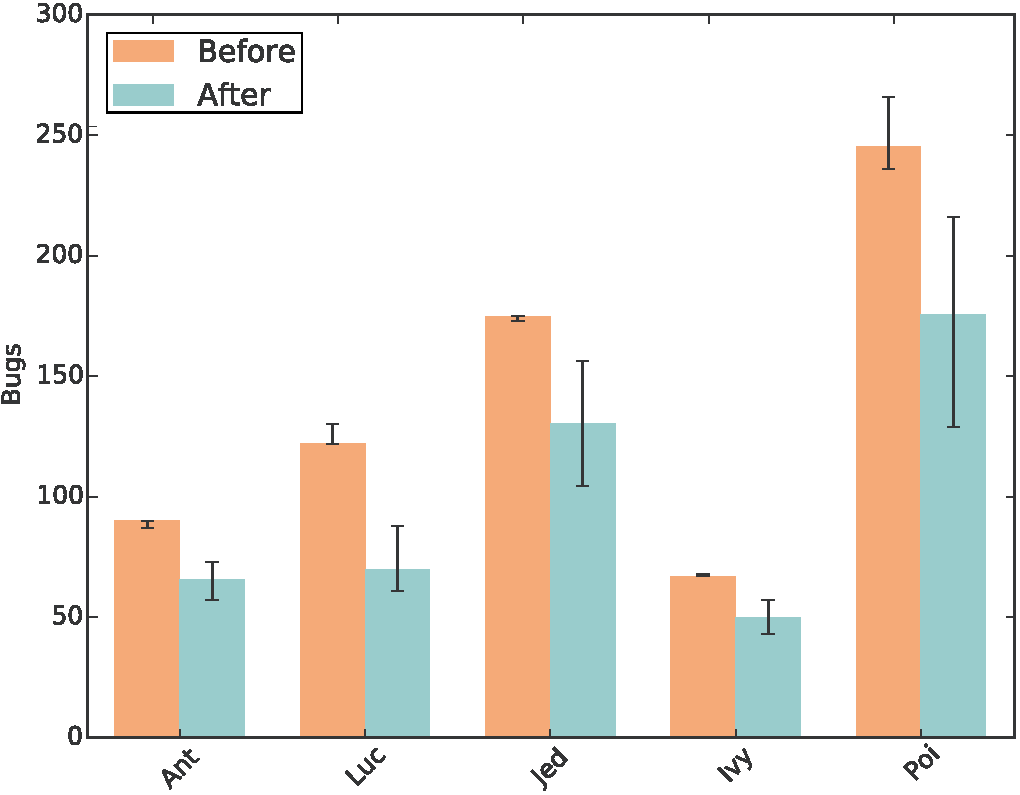
\includegraphics[width=\linewidth]{_figs/histograms.pdf}
\caption{Jureczko object-oriented defect data sets. 
Comparisons of predictions of defects in the Jureczko data sets before and after planning.}
\label{fig:bugs}
\end{figure}

\subsection{Visualisations of Changes}

In this section, we show some sample results. In the next section, we conduct a statistical
analysis of all   results.

\fig{bugs} shows the effects of planning on the five good Jureczko data sets. Note that:
\bi
\item
The number of defects predicted in the ``after'' set is always less than ``before'';
\item
The reduction can be quite large: e.g. see the over 50\% reduction in the {\em ant} data set.
\ei

 \begin{figure*}[htbp!]
\centering
\begin{minipage}{0.30\linewidth}
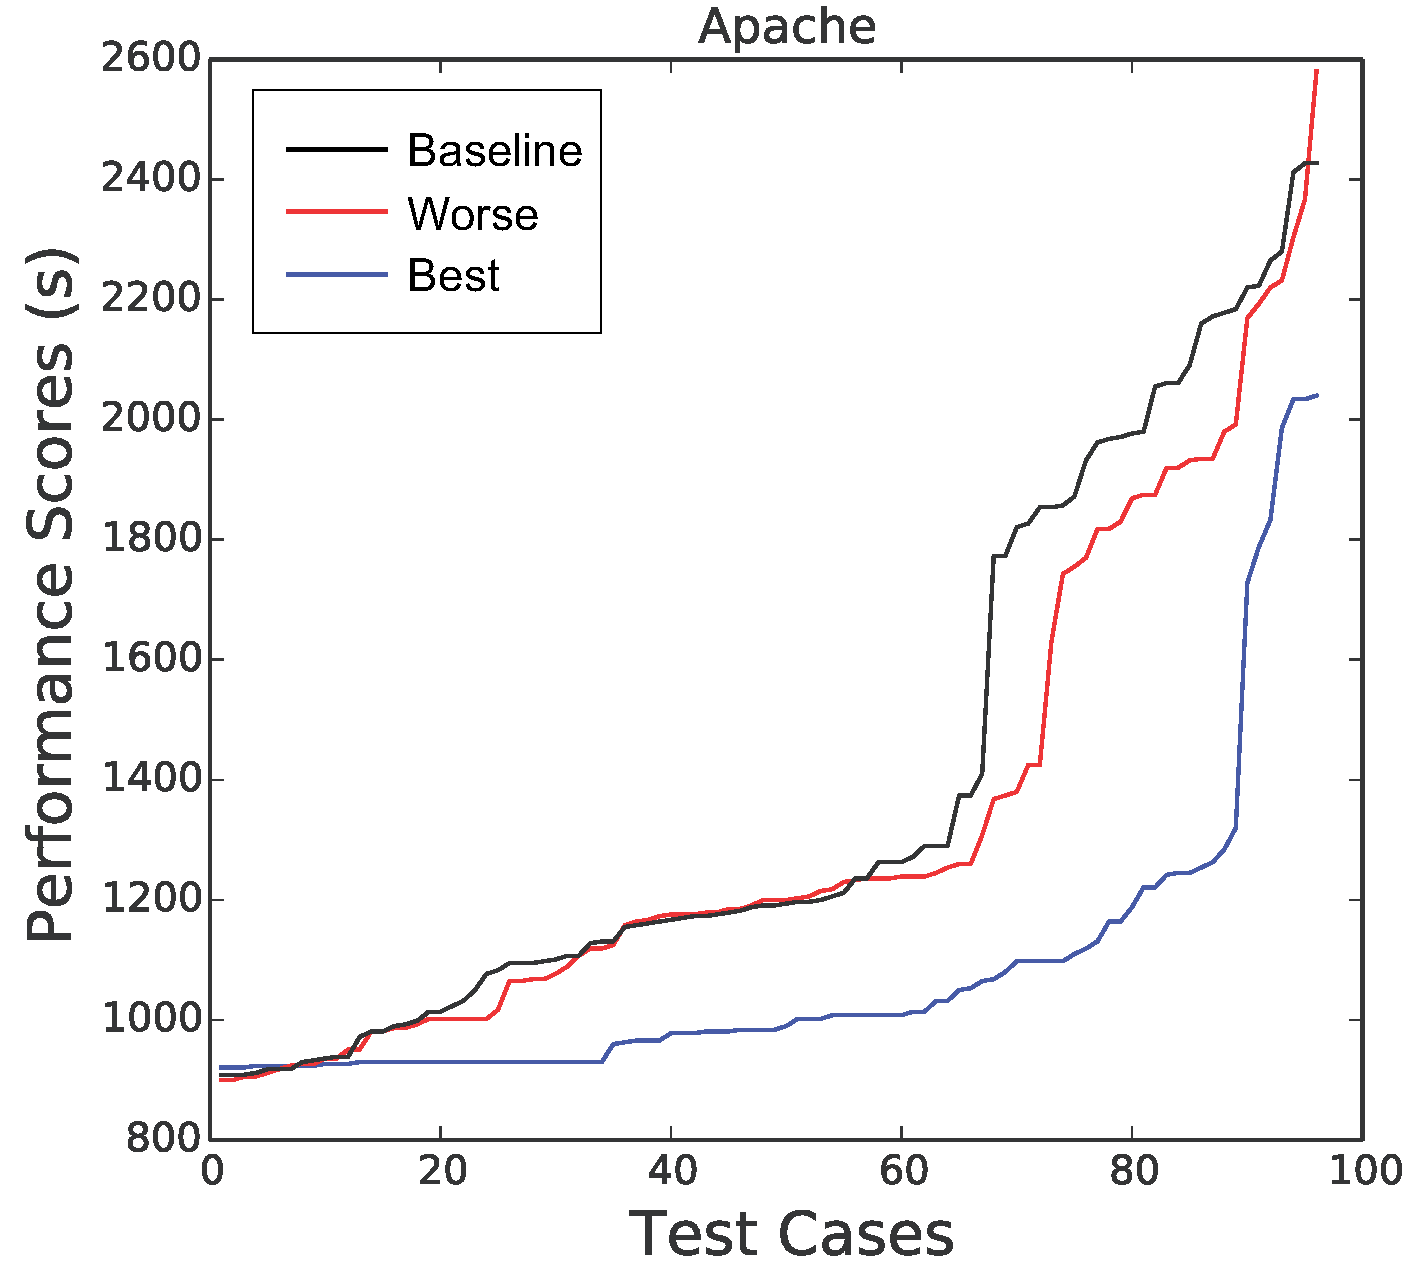
\includegraphics[width=\linewidth]{_figs/Apache.pdf}
\end{minipage}
\begin{minipage}{0.30\linewidth}
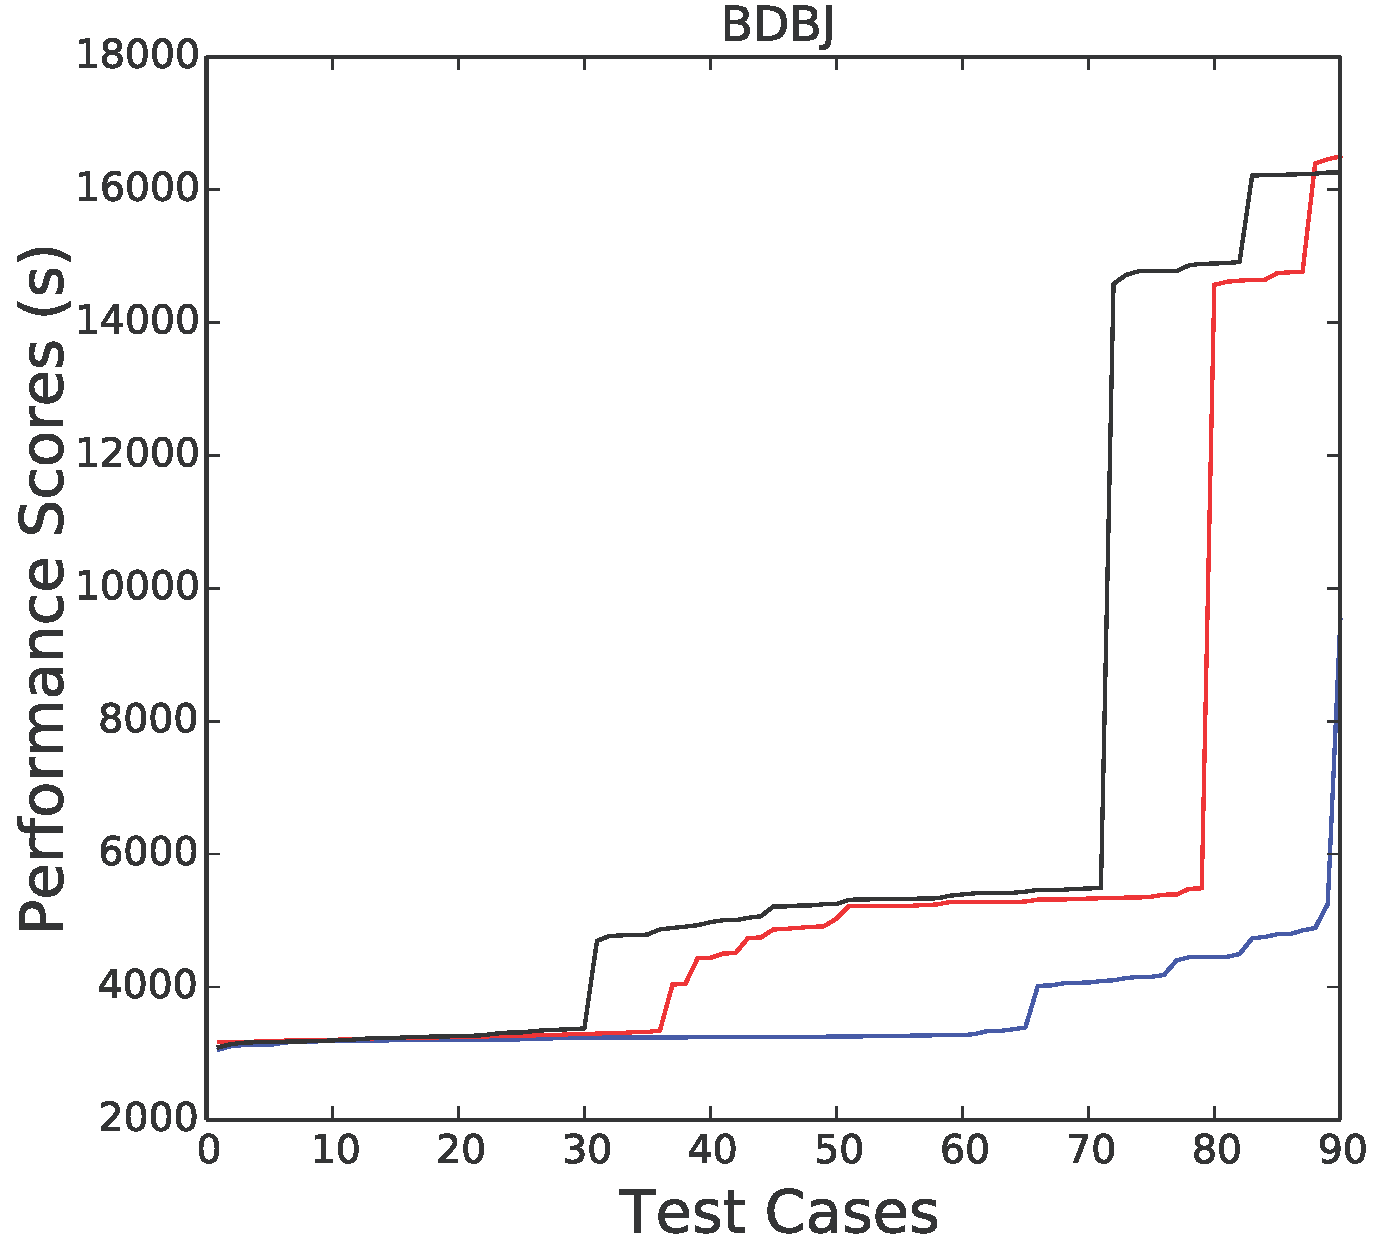
\includegraphics[width=\linewidth]{_figs/BDBJ.pdf}
\end{minipage}
\begin{minipage}{0.30\linewidth}
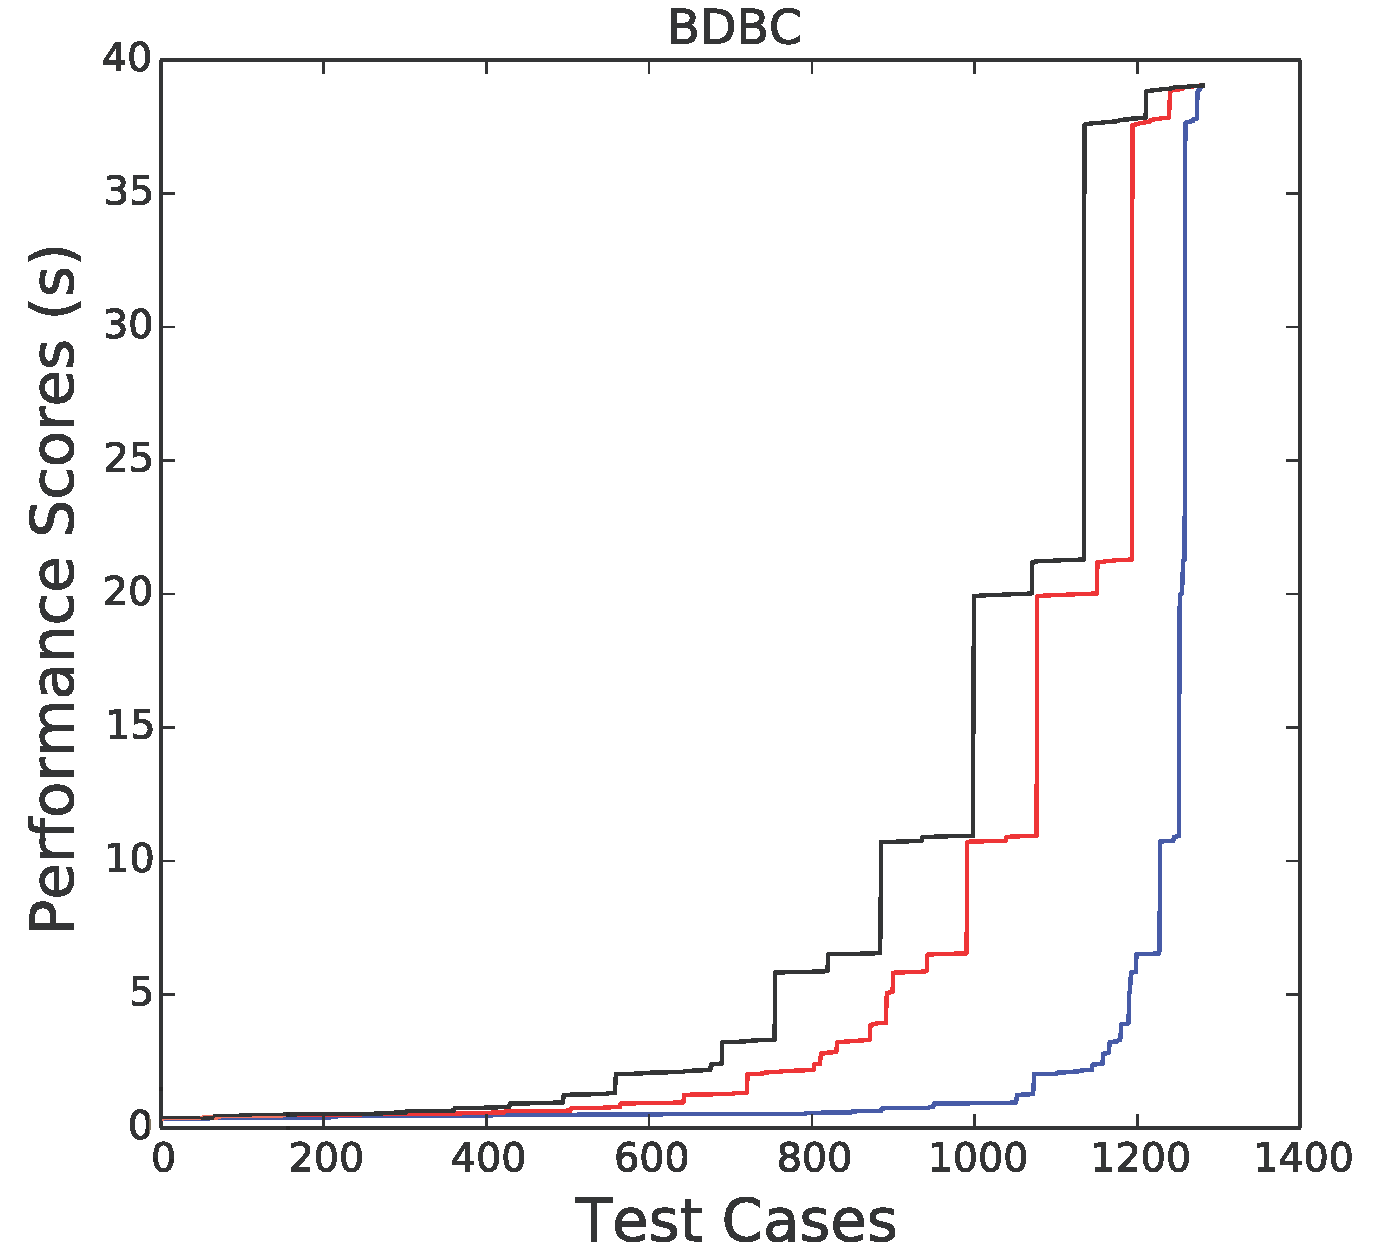
\includegraphics[width=\linewidth]{_figs/BDBC.pdf}
\end{minipage}\\[0.25cm]

\begin{minipage}{0.30\linewidth}
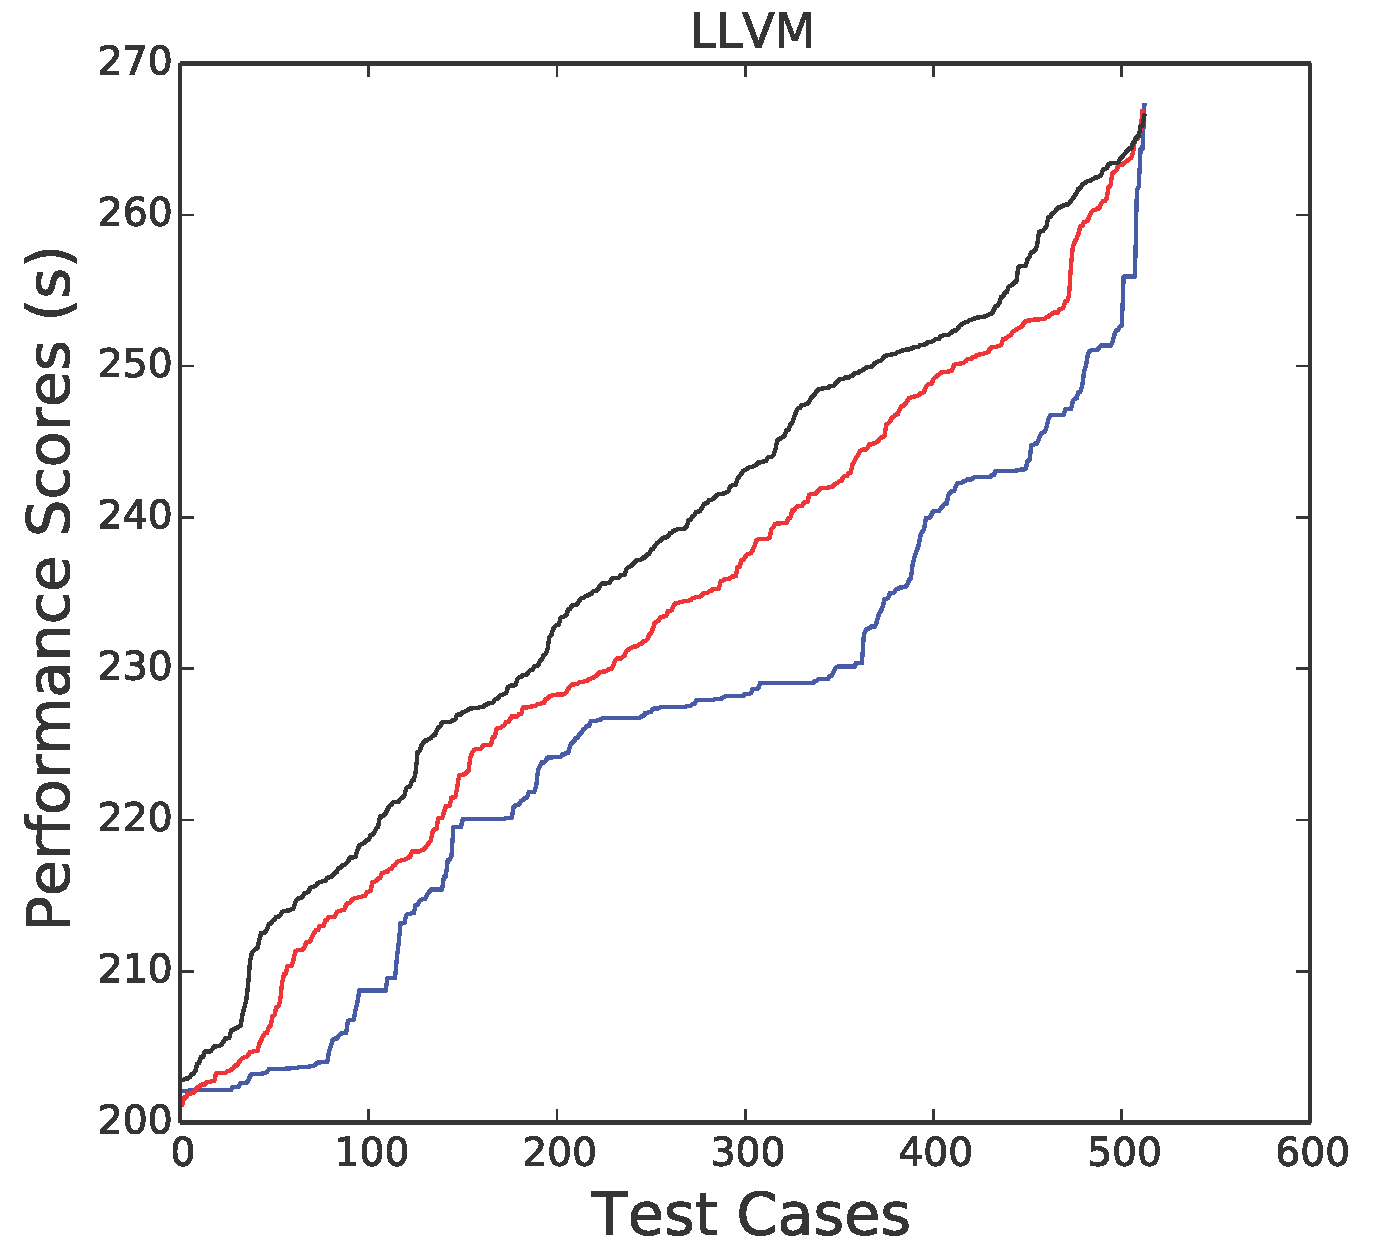
\includegraphics[width=\linewidth]{_figs/LLVM.pdf}
\end{minipage}
\begin{minipage}{0.30\linewidth}
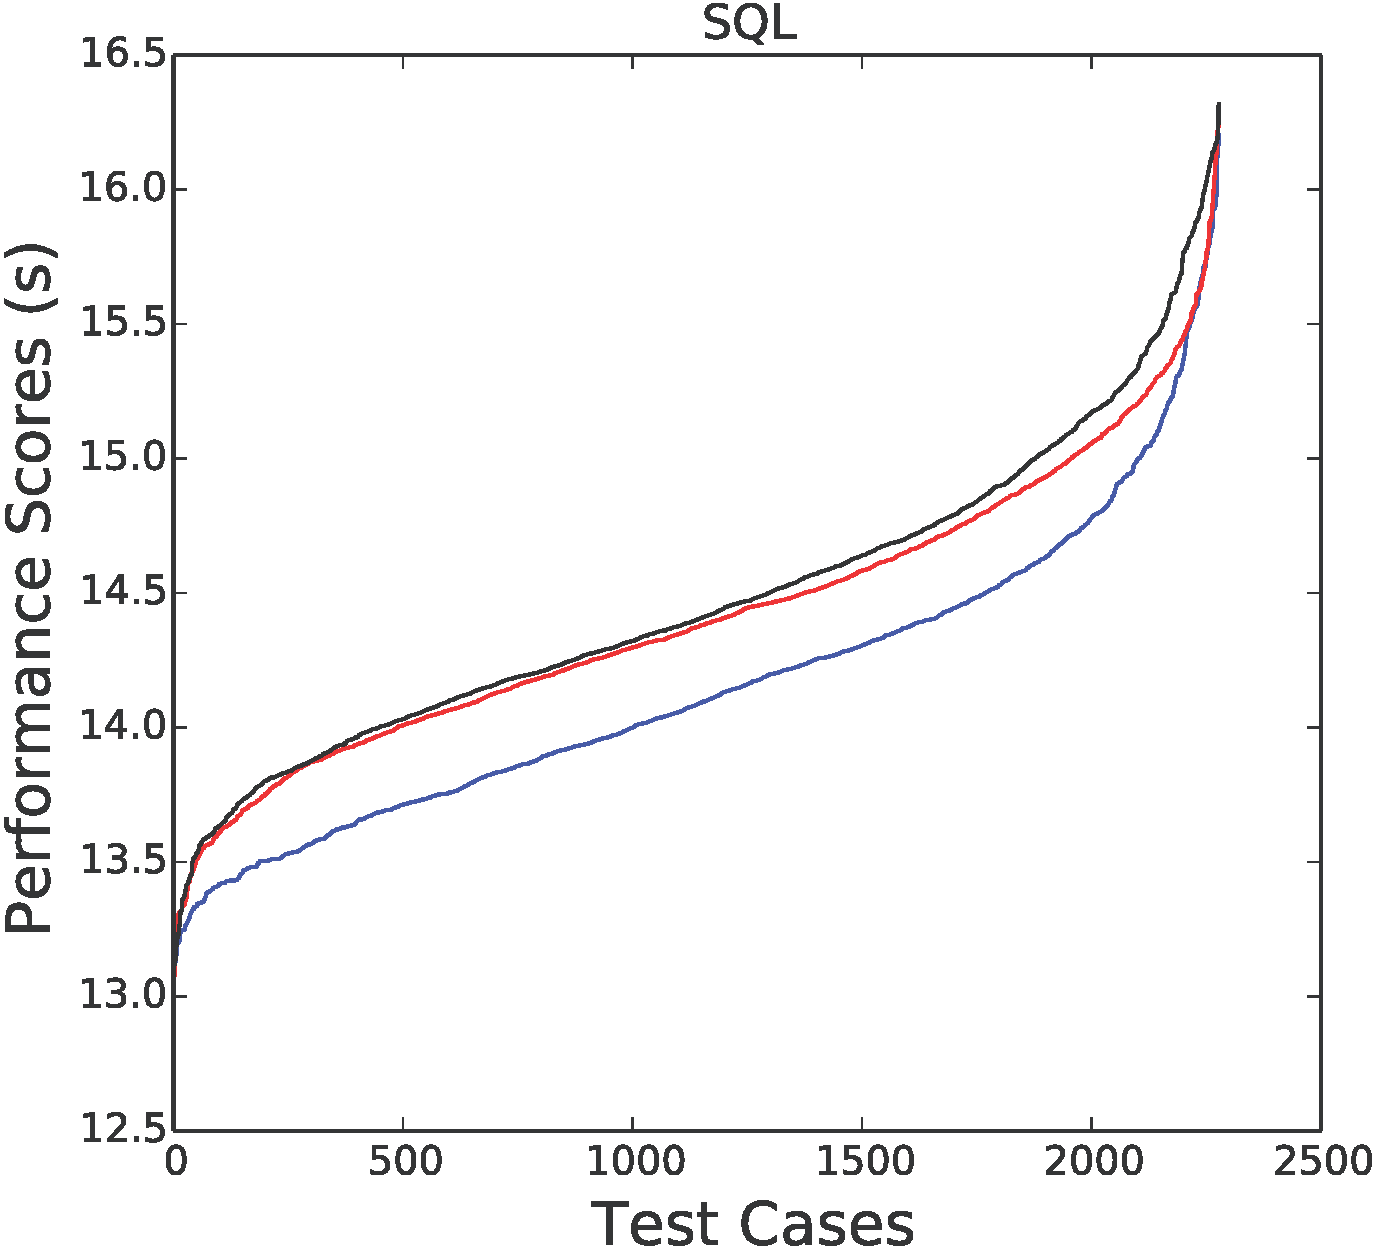
\includegraphics[width=\linewidth]{_figs/SQL.pdf}
\end{minipage}
\begin{minipage}{0.30\linewidth}
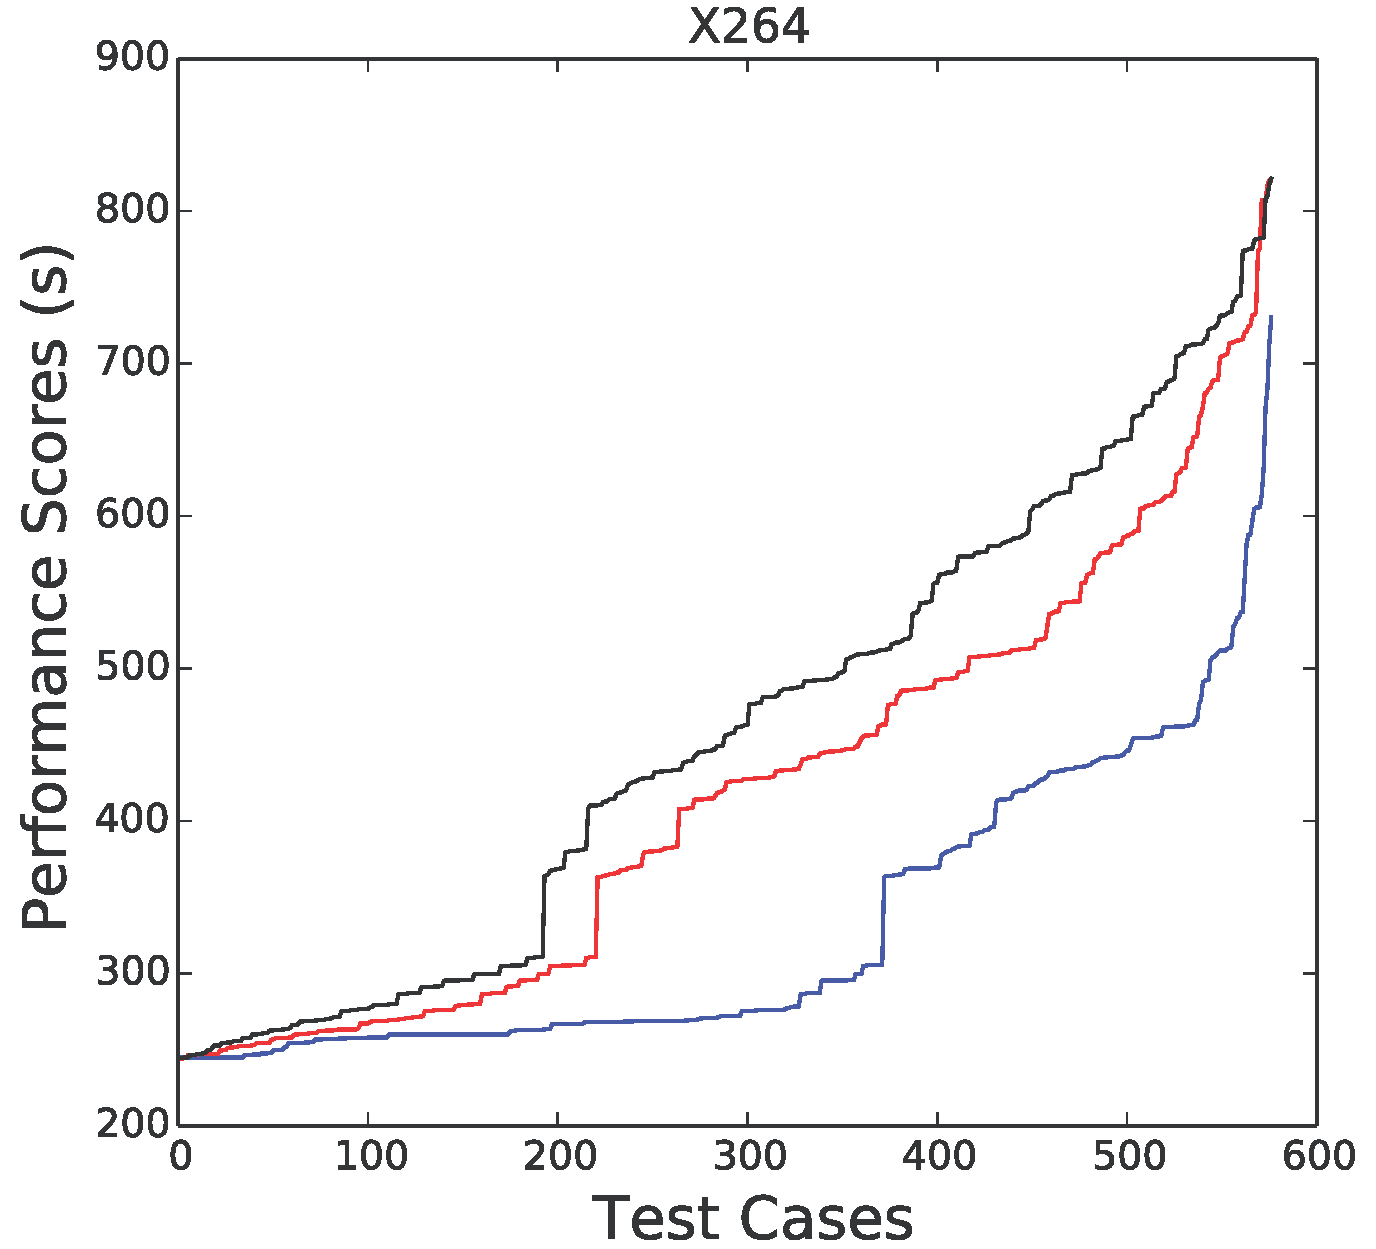
\includegraphics[width=\linewidth]{_figs/X264.pdf}
\end{minipage}
\caption{Run time optimization using HERE . Blue curve represents a mutation probability of 0.75 with feature weighting and information pruning; Red curve represents a mutation probability of 0.25 with feature weighting, but no information pruning; Black curve represents the raw test data used as baseline for the comparison.}
\label{fig:pp}
\end{figure*}

\fig{pp} shows the effects of planning on the Seigmund data sets. The black, red %XXX
curves show the
runtimes as predicted in the test sets before/after our planning.  While some of the differences
are small (eg. LLVM and SQL), some of the others are very large indeed (e.g. the Apache and   BD*).
 
This visual samples of HOW's planning results look promising-- but they need to be confirmed by a
 more rigorous statistical analysis.
 
\subsection{Statistical Analysis}

HOW's performance can be adjusted in numerous ways:
\bi
\item The $F$ variable controls the size of the displacement;
\item The $B$ variable controls how many of the attributes are displaced;
\item The $w_i$ weight inside our distance calcylation controls how important are each variable in computing
     the space between instances. A standard default is $w_i=1$ but this can be adjusted via
     the {\tt featureWeighting} procedure of \fig{howcode}.
\ei

To understand how much (if at all) these variables change the planning results, 
this study ranks methods using the Scott-Knott
procedure recommended by Mittas \& Angelis in their 2013
IEEE TSE paper~\cite{mittas13}.  This method
sorts a list of $l$ treatments with $ls$ measurements by their median
score. It then
splits $l$ into sub-lists $m,n$ in order to maximize the expected value of
 differences  in the observed performances
before and after divisions. E.g. for lists $l,m,n$ of size $ls,ms,ns$ where $l=m\cup n$:
 $E(\Delta)=\frac{ms}{ls}abs(m.\mu - l.\mu)^2 + \frac{ns}{ls}abs(n.\mu - l.\mu)^2$.
Scott-Knott then applies some statistical hypothesis test $H$ to check
if $m,n$ are significantly different. If so, Scott-Knott then recurses on each division.
 
For this study, our hypothesis test $H$ was a
conjunction of the A12 effect size test of  a
non-parametric bootstrap sampling; i.e. our
Scott-Knott divided the data if {\em both}
bootstrapping and an effect size test agreed that
the division was statistically significant (99\%
confidence) and not a ``small'' effect ($A12 \ge
0.6$).
For a justification of the use of non-parametric
bootstrapping, see Efron \&
Tibshirani~\cite[p220-223]{efron93}.
For a justification of the use of effect size tests
see Shepperd\&MacDonell~\cite{shepperd12a}; Kampenes~\cite{kampenes07}; and
Kocaguenli et al.~\cite{kocharm13}. These researchers
warn that even if an
hypothesis test declares two populations to be
``significantly'' different, then that result is
misleading if the ``effect size'' is very small.
Hence, to assess 
the performance differences 
we first must rule out small effects.
This test was recently 
endorsed by Arcuri and Briand
at ICSE'11~\cite{arcuri11}.

 
  



To get an overall count of the   in  order to avoid any parametric bias,
we use the Cliffs Delta score to measure the probability that performance has been changed
by the planner.   Given the untreated test data labeled \textit{Before} of length \textit{M} and the treated instances labeled \textit{After}, the delta score is obtained as follows:
\begin{equation}
\delta = \frac{\#(Before<After) - \#(Before>After)}{M^2}
\label{eq:cliffs}
\end{equation}

A $\delta$ of  0 implies no change at all and, according to Romano et al.~\cite{romano06}, a value less
that 14]7\% is a ``small'' (i.e. negliable) effect.

\begin{figure}[htbp!]

\noindent\begin{minipage}{0.5\textwidth}
  {\scriptsize \textbf{Ant}\\[0.1cm]}
  {\scriptsize  \begin{tabular}{{l@{~~~~}l@{}r@{~~~~}r@{~~~~~}c@{}r}}
      \arrayrulecolor{darkgray}
      \rowcolor[gray]{.9} \textbf{Rank} & \textbf{Treatment} & \textbf{Median} & \textbf{IQR} && \textbf{Bugs}\\
  1 &  0.75-weight &    0.71  &  0.19 & \quart{0}{25}{10}{49} & 62\\
  1 &         0.75 &    0.72  &  0.14 & \quart{6}{19}{12}{49} & 64\\
\hline  2 &          0.5 &    0.86  &  0.08 & \quart{25}{11}{31}{49} & 77 \\
  2 &   0.5-weight &    0.88  &  0.14 & \quart{20}{19}{33}{49} & 77\\
\hline  3 & 0.5-weight-B=50\% &    0.91  &  0.08 & \quart{32}{11}{37}{49} & 80\\
  3 & 0.75-weight-B=50\% &    0.92  &  0.09 & \quart{31}{12}{39}{49} & 82\\
  3 &  0.25-weight &    0.92  &  0.04 & \quart{36}{5}{39}{49} & 81\\
\hline  4 &         0.25 &    0.93  &  0.05 & \quart{37}{7}{40}{49} & 83\\
  4 & 0.75-weight-B=25\% &    0.94  &  0.09 & \quart{36}{12}{41}{49} & 82\\
\hline  5 & 0.25-weight-B=50\% &    0.97  &  0.03 & \quart{44}{4}{45}{49} & 86\\
  5 & 0.5-weight-B=25\% &    0.98  &  0.06 & \quart{40}{8}{47}{49} & 86 \\
\hline  6 & 0.25-weight-B=25\% &    0.99  &  0.01 & \quart{48}{1}{48}{49} & 87\\
\hline  7 &         Base &    1.0  &  0.0 & \quart{49}{0}{49}{49} & 90\\
\hline \end{tabular}}
\end{minipage}\\[0.1cm] 

\noindent\begin{minipage}{0.5\textwidth}
  \flushleft
  {\scriptsize \textbf{Ivy}\\[0.1cm]}
{\scriptsize  \begin{tabular}{{l@{~~~~}l@{}r@{~~~~}r@{~~~~}c@{}r}}
\arrayrulecolor{darkgray}
\rowcolor[gray]{.9} \textbf{Rank} & \textbf{Treatment} & \textbf{Median} & \textbf{IQR} & & \textbf{Bugs}\\
  1 &  0.75-weight &    0.75  &  0.18 & \quart{0}{29}{8}{49} & 50\\
  1 &         0.75 &    0.79  &  0.12 & \quart{8}{20}{14}{49} & 53\\
\hline  2 &          0.5 &    0.84  &  0.1 & \quart{18}{16}{23}{49} & 56\\
  2 &   0.5-weight &    0.84  &  0.08 & \quart{14}{14}{23}{49} & 56\\
  2 & 0.75-weight-B=50\% &    0.84  &  0.09 & \quart{18}{15}{23}{49} & 56 \\
\hline  3 & 0.5-weight-B=50\% &    0.91  &  0.05 & \quart{29}{9}{34}{49} & 61\\
\hline  4 & 0.25-weight-B=50\% &    0.96  &  0.01 & \quart{43}{1}{43}{49} & 64\\
  4 & 0.75-weight-B=25\% &    0.96  &  0.05 & \quart{39}{9}{43}{49} & 65\\
  4 &         0.25 &    0.97  &  0.01 & \quart{43}{1}{44}{49} & 65\\
  4 &  0.25-weight &    0.97  &  0.05 & \quart{39}{9}{44}{49} & 65 \\
  4 & 0.5-weight-B=25\% &    0.97  &  0.03 & \quart{43}{5}{44}{49} & 65 \\
\hline  5 & 0.25-weight-B=25\% &    0.99  &  0.01 & \quart{48}{1}{48}{49} & 66\\
\hline  
6 &         Base &    1.0  &  0.0 & \quart{49}{0}{49}{49} & 67\\
\hline \end{tabular}}
\end{minipage}\\[0.1cm] 

\noindent\begin{minipage}{0.5\textwidth}
  \flushleft
  {\scriptsize \textbf{Jedit}\\[0.1cm]}
  {\scriptsize  \begin{tabular}{{l@{~~~~}l@{}r@{~~~~}r@{~~~~}c@{}r}}
\arrayrulecolor{darkgray}
\rowcolor[gray]{.9} \textbf{Rank} & \textbf{Treatment} & \textbf{Median} & \textbf{IQR} & & \textbf{Bugs}\\\hline
  1 &         0.75 &    0.64  &  0.28 & \quart{0}{27}{14}{49} & 110\\
\hline  2 &  0.75-weight &    0.76  &  0.21 & \quart{13}{21}{26}{49}& 131 \\
  2 &   0.5-weight &    0.76  &  0.16 & \quart{20}{16}{26}{49} & 130\\
  2 &          0.5 &    0.79  &  0.17 & \quart{19}{17}{29}{49} & 137\\
\hline  3 & 0.75-weight-B=50\% &    0.85  &  0.12 & \quart{30}{12}{35}{49} & 146\\
  3 &  0.25-weight &    0.87  &  0.07 & \quart{34}{7}{37}{49} & 152\\
\hline  4 &         0.25 &    0.93  &  0.09 & \quart{37}{9}{43}{49} & 161\\
  4 & 0.5-weight-B=50\% &    0.93  &  0.05 & \quart{41}{5}{43}{49} & 162\\
\hline  5 & 0.25-weight-B=50\% &    0.97  &  0.03 & \quart{45}{3}{47}{49} & 167\\
  5 & 0.75-weight-B=25\% &    0.97  &  0.02 & \quart{46}{2}{47}{49} & 168\\
\hline  6 & 0.5-weight-B=25\% &    0.98  &  0.02 & \quart{47}{2}{48}{49} & 170\\
  6 & 0.25-weight-B=25\% &    0.98  &  0.01 & \quart{48}{1}{48}{49} & 171\\
\hline  7 &         Base &    1.0  &  0.0 & \quart{49}{0}{49}{49} & 175\\
\hline \end{tabular}}
\end{minipage}\\[0.1cm] 

\noindent\begin{minipage}{0.5\textwidth}
  \flushleft
  {\scriptsize \textbf{Lucene}\\[0.1cm]}
  {\scriptsize  \begin{tabular}{{l@{~~~~}l@{}r@{~~~~}r@{~~~~}c@{}r}}
\arrayrulecolor{darkgray}
\rowcolor[gray]{.9} \textbf{Rank} & \textbf{Treatment} & \textbf{Median} & \textbf{IQR} & & \textbf{Bugs}\\
  1 &  0.75-weight &    0.66  &  0.2 & \quart{0}{21}{13}{49} & 97 \\
\hline  2 & 0.75-weight-B=50\% &    0.7  &  0.1 & \quart{14}{10}{17}{49} & 103 \\
\hline  3 &         0.75 &    0.77  &  0.3 & \quart{9}{33}{24}{49} & 113\\
  3 & 0.75-weight-B=25\% &    0.8  &  0.09 & \quart{21}{10}{28}{49} & 117\\
  3 &   0.5-weight &    0.81  &  0.09 & \quart{26}{9}{29}{49} & 119\\
  3 &          0.5 &    0.84  &  0.1 & \quart{26}{10}{32}{49} & 123\\
\hline  4 & 0.5-weight-B=50\% &    0.88  &  0.07 & \quart{34}{8}{36}{49} & 128\\
  4 & 0.25-weight-B=25\% &    0.89  &  0.07 & \quart{36}{8}{38}{49} & 130 \\
  4 &  0.25-weight &    0.92  &  0.04 & \quart{39}{4}{41}{49} & 133 \\
  4 &         0.25 &    0.93  &  0.07 & \quart{36}{8}{42}{49} & 136 \\
\hline  5 & 0.25-weight-B=50\% &    0.95  &  0.04 & \quart{42}{4}{44}{49} & 139 \\
  5 & 0.5-weight-B=25\% &    0.96  &  0.03 & \quart{43}{3}{45}{49} &141 \\
\hline  6 &         Base &    1.0  &  0.0 & \quart{49}{0}{49}{49} & 146\\
\hline \end{tabular}}
\end{minipage}\\[0.1cm] 

\noindent\begin{minipage}{0.5\textwidth}
  \flushleft
  {\scriptsize \textbf{Poi}\\[0.1cm]}
  {\scriptsize  \begin{tabular}{{l@{~~~~}l@{}r@{~~~~}r@{~~~~}c@{}r}}
      \arrayrulecolor{darkgray}
\rowcolor[gray]{.9} \textbf{Rank} & \textbf{Treatment} & \textbf{Median} & \textbf{IQR} & & \textbf{Bugs}\\
  1 &  0.75-weight &    0.72  &  0.26 & \quart{0}{29}{18}{49} & 173\\
  1 &         0.75 &    0.74  &  0.18 & \quart{12}{20}{20}{49} & 178\\
\hline  2 & 0.75-weight-B=50\% &    0.79  &  0.15 & \quart{14}{17}{26}{49} & 190\\
  2 &          0.5 &    0.81  &  0.15 & \quart{22}{17}{28}{49} & 195\\
  2 &   0.5-weight &    0.81  &  0.14 & \quart{21}{16}{28}{49} & 195\\
\hline  3 & 0.5-weight-B=50\% &    0.9  &  0.11 & \quart{30}{13}{38}{49} & 217\\
  3 &         0.25 &    0.91  &  0.07 & \quart{35}{8}{39}{49} & 219\\
  3 &  0.25-weight &    0.91  &  0.05 & \quart{36}{6}{39}{49} & 219\\
\hline  4 & 0.75-weight-B=25\% &    0.94  &  0.05 & \quart{39}{6}{43}{49} & 226\\
  4 & 0.25-weight-B=50\% &    0.94  &  0.06 & \quart{39}{7}{43}{49} & 226\\
\hline  5 & 0.25-weight-B=25\% &    0.96  &  0.03 & \quart{44}{3}{45}{49} & 231\\
  5 & 0.5-weight-B=25\% &    0.96  &  0.03 & \quart{44}{3}{45}{49} & 231\\
\hline  6 &         Base &    1.0  &  0.0 & \quart{49}{0}{49}{49} & 240 \\
\hline \end{tabular}}
\end{minipage}
\caption{Cliffs Delta Scores for the defect data set. The Treatment column, has 3 possible configurations, the first (0.25, 0.50, and 0.75) represents the extent of mutation; weighting represents feature weighting; Prune represents the extent of information pruning.}
\label{tab:ant}
\end{figure}

\subsection{Performance Prediction Data set}

In this section, 
\begin{figure*}[htbp!]
\noindent\begin{minipage}{0.5\textwidth}
  {\scriptsize \textbf{Apache}\\}
  {\scriptsize  \begin{tabular}{{l@{~~~~}l@{~~~~}r@{~~~~}r@{~~~~}c}}
      \arrayrulecolor{darkgray}
      \rowcolor[gray]{.9} \textbf{Rank} & \textbf{Treatment} & \textbf{Median} & \textbf{IQR} & \\
  1 & 0.75-weight-B=25\% &    0.77  &  0.05 & \quart{0}{14}{5}{74}\\
  1 &  0.75 &    0.79  &  0.08 & \quart{2}{24}{11}{74}\\
\hline  2 & 0.75-weight &    0.85  &  0.07 & \quart{14}{21}{29}{74}\\
  2 & Apache\_50\_w\_iP(25) &    0.85  &  0.04 & \quart{23}{12}{29}{74}\\
  2 &  Apache\_50 &    0.85  &  0.05 & \quart{26}{15}{29}{74}\\
\hline  3 & Apache\_50\_w &    0.91  &  0.05 & \quart{38}{15}{47}{74}\\
\hline  4 &  Apache\_25 &    0.92  &  0.04 & \quart{44}{12}{50}{74}\\
  4 & Apache\_25\_w\_iP(25) &    0.93  &  0.02 & \quart{50}{6}{53}{74}\\
\hline  5 & Apache\_25\_w &    0.96  &  0.03 & \quart{56}{9}{62}{74}\\
\hline  6 & Apache\_baseline &    1.0  &  0.0 & \quart{74}{0}{74}{74}\\\hline \end{tabular}}
\end{minipage}
\noindent\begin{minipage}{0.5\textwidth}
  \flushleft
  {\scriptsize \textbf{BDBC}\\}
{\scriptsize  \begin{tabular}{{l@{~~~~}l@{~~~~}r@{~~~~}r@{~~~~}c}}
\arrayrulecolor{darkgray}
\rowcolor[gray]{.9} \textbf{Rank} & \textbf{Treatment} & \textbf{Median} & \textbf{IQR} & \\
  1 &     75 &    0.22  &  0.05 & \quart{0}{3}{1}{49} \\
  1 &  75, weighting, Prune=25\% &    0.21  &  0.04 & \quart{0}{2}{0}{49} \\
\hline  2 &  75, weighting &    0.24  &  0.1 & \quart{0}{6}{2}{49} \\
\hline  3 &     50 &    0.4  &  0.04 & \quart{11}{2}{12}{49} \\
  3 &  50, weighting, Prune=25\% &    0.4  &  0.05 & \quart{10}{3}{12}{49} \\
\hline  4 &  50, weighting &    0.47  &  0.09 & \quart{14}{5}{16}{49} \\
\hline  5 &     25 &    0.66  &  0.03 & \quart{28}{1}{28}{49} \\
  5 &  25, weighting, Prune=25\% &    0.67  &  0.06 & \quart{28}{3}{29}{49} \\
\hline  6 &  25, weighting &    0.69  &  0.06 & \quart{29}{4}{30}{49} \\
\hline  7 &  baseline &    1.0  &  0.0 & \quart{49}{0}{49}{49} \\
\hline \end{tabular}}
\end{minipage}

\noindent\begin{minipage}{0.5\textwidth}
  \flushleft
  {\scriptsize \textbf{BDBJ}\\}
{\scriptsize  \begin{tabular}{{l@{~~~~}l@{~~~~}r@{~~~~}r@{~~~~}c}}
\arrayrulecolor{darkgray}
\rowcolor[gray]{.9} \textbf{Rank} & \textbf{Treatment} & \textbf{Median} & \textbf{IQR} & \\
  1 &     75 &    0.63  &  0.16 & \quart{0}{19}{3}{49} \\
  1 &  75, weighting, Prune=25\% &    0.68  &  0.17 & \quart{1}{21}{9}{49} \\
  1 &  75, weighting &    0.74  &  0.11 & \quart{8}{14}{17}{49} \\
\hline  2 &  50, weighting, Prune=25\% &    0.75  &  0.09 & \quart{14}{12}{18}{49} \\
  2 &     50 &    0.79  &  0.13 & \quart{16}{16}{23}{49} \\
\hline  3 &  50, weighting &    0.82  &  0.09 & \quart{23}{11}{27}{49} \\
\hline  4 &  25, weighting, Prune=25\% &    0.87  &  0.07 & \quart{29}{9}{33}{49} \\
\hline  5 &     25 &    0.88  &  0.06 & \quart{33}{8}{34}{49} \\
  5 &  25, weighting &    0.92  &  0.06 & \quart{36}{7}{39}{49} \\
\hline  6 &  baseline &    1.0  &  0.0 & \quart{49}{0}{49}{49} \\
\hline \end{tabular}}
\end{minipage}
\noindent\begin{minipage}{0.5\textwidth}
  \flushleft
  {\scriptsize \textbf{LLVM}\\}
  {\scriptsize  \begin{tabular}{{l@{~~~~}l@{~~~~}r@{~~~~}r@{~~~~}c}}
\arrayrulecolor{darkgray}
\rowcolor[gray]{.9} \textbf{Rank} & \textbf{Treatment} & \textbf{Median} & \textbf{IQR} & \\
  1 &     75 &    0.92  &  0.01 & \quart{5}{6}{5}{49} \\
  1 &  75, weighting, Prune=25\% &    0.92  &  0.02 & \quart{0}{11}{5}{49} \\
  1 &  75, weighting &    0.93  &  0.02 & \quart{5}{11}{11}{49} \\
\hline  2 &     50 &    0.94  &  0.01 & \quart{16}{6}{16}{49} \\
  2 &  50, weighting, Prune=25\% &    0.95  &  0.0 & \quart{22}{0}{22}{49} \\
  2 &  50, weighting &    0.96  &  0.02 & \quart{22}{11}{27}{49} \\
\hline  3 &     25 &    0.98  &  0.01 & \quart{33}{5}{38}{49} \\
  3 &  25, weighting, Prune=25\% &    0.98  &  0.01 & \quart{33}{5}{38}{49} \\
  3 &  25, weighting &    0.98  &  0.0 & \quart{38}{0}{38}{49} \\
\hline  4 &  baseline &    1.0  &  0.0 & \quart{49}{0}{49}{49} \\
\hline \end{tabular}}
\end{minipage}


\noindent\begin{minipage}{0.5\textwidth}
  \flushleft
  {\scriptsize \textbf{SQL}\\}
  {\scriptsize  \begin{tabular}{{l@{~~~~}l@{~~~~}r@{~~~~}r@{~~~~}c}}
\arrayrulecolor{darkgray}
\rowcolor[gray]{.9} \textbf{Rank} & \textbf{Treatment} & \textbf{Median} & \textbf{IQR} & \\
  1 &      75 &    0.98  &  0.01 & \quart{0}{16}{16}{49} \\
  1 &  75, weighting, Prune=25\% &    0.98  &  0.0 & \quart{16}{0}{16}{49} \\
  1 &  75, weighting &    0.99  &  0.01 & \quart{16}{17}{33}{49} \\
  1 &  50, weighting, Prune=25\% &    0.99  &  0.0 & \quart{33}{0}{33}{49} \\
  1 &      50 &    0.99  &  0.0 & \quart{33}{0}{33}{49} \\
  1 &  50, weighting &    0.99  &  0.01 & \quart{33}{16}{33}{49} \\
  1 &  25, weighting, Prune=25\% &    1.0  &  0.0 & \quart{49}{0}{49}{49} \\
  1 &      25 &    1.0  &  0.0 & \quart{49}{0}{49}{49} \\
  1 &  25, weighting &    1.0  &  0.0 & \quart{49}{0}{49}{49} \\
  1 &  baseline &    1.0  &  0.0 & \quart{49}{0}{49}{49} \\
  \hline \end{tabular}}
\end{minipage}
\noindent\begin{minipage}{0.5\textwidth}
  \flushleft
  {\scriptsize \textbf{X264}\\}
  {\scriptsize  \begin{tabular}{{l@{~~~~}l@{~~~~}r@{~~~~}r@{~~~~}c}}
\arrayrulecolor{darkgray}
\rowcolor[gray]{.9} \textbf{Rank} & \textbf{Treatment} & \textbf{Median} & \textbf{IQR} & \\
  1 &  75, weighting, Prune=25\% &    0.73  &  0.05 & \quart{1}{9}{3}{49} \\
  1 &     75 &    0.74  &  0.05 & \quart{0}{8}{5}{49} \\
\hline  2 &  75, weighting &    0.81  &  0.04 & \quart{13}{7}{17}{49} \\
  2 &  50, weighting, Prune=25\% &    0.82  &  0.04 & \quart{17}{7}{18}{49} \\
  2 &     50 &    0.83  &  0.03 & \quart{17}{5}{20}{49} \\
\hline  3 &  50, weighting &    0.88  &  0.03 & \quart{25}{6}{29}{49} \\
\hline  4 &     25 &    0.9  &  0.03 & \quart{31}{5}{32}{49} \\
  4 &  25, weighting, Prune=25\% &    0.91  &  0.03 & \quart{32}{5}{34}{49} \\
\hline  5 &  25, weighting &    0.93  &  0.02 & \quart{36}{3}{37}{49} \\
\hline  6 &  baseline &    1.0  &  0.0 & \quart{49}{0}{49}{49} \\
\hline \end{tabular}}
\end{minipage}
\end{figure*}


% \section{Discussion}
\section{Threats to validity}

 

As with any empirical study, biases can affect the final results. Therefore, any
conclusions made from this work must be considered with the following issues in
mind.

{\em 1. Sampling bias} threatens any data mining experiment; i.e., what matters
there may not be true here. For example, the data sets used here comes from two sources
(Seigmund et al. and Jureczko et al.) and any biases in their selection procedures
threaten the validity of these results. 
That said,
the best we can do is define our methods and publicize our data and code so that other researchers can
try to repeat our results and, perhaps, point out a previously unknown bias
in our analysis. Hopefully, other researchers will emulate our methods in
order to repeat, refute, or improve our results. 

{\em 2. Learner bias: } For building the defect predictors in this study, we elected
to use  Random Forest  .
We chose Random Forest based on its reputation for having the better  performance of 
21 other learners for defect prediction~\cite{lessmann}.
Data mining is a
large and active field and any single study can only use a small
subset of the known classification algorithms.  

{\em 3. Evaluation bias:} The issue was discussed above in \tion{assess} where
we asserted that plans can be assessed via predictors-- with the all important
proviso that the planning should {\em not} be attempted if the predictors
are performing poorly.

%%\footnote{LL: It seems to me that $privacy$ in LACE approach could be compromised in the case of extremes if I had some knowledge of the parties. Consider a case where you know that a bunch of startups and Microsoft contributed to a private cache. Even with the random perturbation in MORPH, it will be REALLY obvious which defect data came from Windows vs. all of the others because Windows will have LOC orders of magnitude greater than anyone else, right?}
 
%XXXX everytime it says LACE, do you mean LACE2

%{\em 4. Comparison bias:}
%There are many privacy algorithms~\cite{Fung2010survey} and it would be difficult to 
%compare their performances (especially with various ways to measure privacy).
%In this work, we use LACE.

%{\em 5. Other Evaluation Bias:}
%The utility of  obfuscated data can be measured
%semantically (where the workload is unknown) or empirically (known workload
%e.g., classification or aggregate query answering). In this work we measure
%utility empirically for defect prediction only.


%

\section{Related Work}
The connection of HOW to model-based evolutionary programming was discussed above.
In summary,   model-based tools such as NSGA-III~\cite{deb14} or MOEA/D~\cite{zhang07:TEC}
use some domain model as part of extensive Monte Carlo studies (augmented with some
evolution of selected best instances).
The premise of HOW is that we have access to domain data, but not a domain model.
Also, the results shown above were obtained without evolving/updating some current population
multiple times.


Planning with HERE is somewhat different to the recommendor systems.
As described by Robillard and Walker~\cite{rob14}, recommendor systems
in software engineering
are less {\em directive} and more    {\em collaborative} than policy
generators:
\bi
\item
Directive systems such as HERE tell developers exactly what to do
(e.g. ``use these settings in a Makefile'') 
\item
The collaborative systems discussed by Robillard and Walker
are more suggestive guides that
help (e.g.) programmers focus on very small sets
with  very large libraries of code of documentation.
\ei
One difference between directive and collaborative systems is that
the latter may not presume to suggest exactly what to do next.
However, planning systems like HOW are much more ardent: then make precise recommendations
of how to change all items in the test suite.
 

HOW is more a data mining method than a model-based optimizer. It represents our next attempt
to develop model-less instance-based optimizers.  Our previous attempts in this area
were the W2, WHERE, and IDEA systems~~\cite{menzies13:brady,Menzies2013:local,me12c}.
W2 was developed with Brady et al.~\cite{menzies13:brady}. 
W2 reasoned over deltas in the the raw
attributes values (and not the synthesized attributes used by HOW). 
The results of  adjusting values via those deltas was assessed via an SQL-like
query that selected all examples in the database that satisfied the newly adjusted
values. W2 suffers from two problems that are resolved
in this paper: {\em optimization failure} and {\em instance exhastion}.
\bi
\item 
As reported in that paper, W2
had a large number of {\em optimization failures}; i.e. after applying its recommendations,
the objective scores actually got worse. We recommend HOW's approach (of reasoning
over the synthesized attributes) to W2 since {\em in none of the above
results} do we observe that {\em after} we treat the data, that the objective scores are worse.
\item
As to {\em instance exhaustion}, W2 was a simple case-based reasoning system that never generalized
over its instances. Hence, the SQl-like query used to asses W2's plans often returned
a vanishingly small number of instances. To avoid this problem, we strongly recommend
combining a planning system with a prediction system (as done in this paper) such that we can
generalize to adjusted examples not seen on the original sample.
\ei
The WHERE tool~\cite{Menzies2013:local} developed the recursive clustering method over synthesized attributes
  used in this paper. WHERE was   a prediction
system since reported current patterns in the data, rather than proposing plans
on how to improve those patterns. Nor did that tool offer guidance on how to assess
the results of stepping along those patterns to guide changes to the system.

The problems of W2 and the success of WHERE suggested in might be useful to combine
WHERE's synthesized attributes with W2. The result was the IDEA tool~\cite{me12c}. 
While the initial prototype seemed promising~\cite{me12c}, we made the mistake of using
the tree structure of the recursive clusters to generate plans (in IDEA, the plan to
move an instance from one poorly performing cluster $C_1$ to another $C_2$ was computed
from the different in the  median
values of the instances in the two  branches that lead to $C_1$ and $C_2$).  When
that approach was applied to the data used in this paper, the results were quite weak
(very little net improvement). However, we abandoned the tree-query approach
and went for the pure instance-based approach discussed at the start of this paper.


Moving on to other releated work, depending on the audience  we would
 call HOW a {\em spectral learner}, 
a {\em response surface method}, or  a {\em local search operator}.
According to
Kamvar et al~\cite{kamvar03}
{\em spectral learners}reason across $m$ underlying dimensions synthesized
using (say) PCA~\cite{pearson1901}. For example,
algorithms like PDDP~\cite{boley98} use PCA to
recursively divide data into smaller regions where each level of recursion needs an   $O(N^2)$ analysis
to infer the principle components. HOW performs an analogous procedure using a   $O(2N)$ analysis
based on a heuristic proposed by
Faloutsos and Lin~\cite{Faloutsos1995} (see above, the ``FASTMAP'' algorithm).

{\em Response surface methods}  build a fast approximation to the function being optimized,
then uses that  approximation to take intelligent guesses about useful mutations. HOW
is a non-parametric response surface method that finds its response surface via recursive
clustering. For an example of a parametric response surface method, that uses Gaussian process
models, see Zuluaga et al.~\cite{zuluaga13}.

A {\em local search operator} that a some probability $p$, nudges  instance variables
along a dimension that improves its objective scores. HOW's recursive clustering methods
combine $n$ dimensions into $m \ll n$ so its ``nudges'' are simultaneous
adjustments along multiple dimensions. For an example of other kinds of local search algorithms, that only adjust
one variable at a time, see the literature on WALKSAT~\cite{Selman1992} and MAXWALKSAT~\cite{kautz97}.
See also the literature on local search methods in multi-objective optimization.
For example,
Peng et al.~\cite{peng09:ls} have augmented MOEAs with
local search  (i.e. applying a problem-specific repair/improvement
heuristic on some current solution).
Also, Igel et al.'s~\cite{igel07} multi-objective
covariance matrix adaptation evolution strategy
can run the mutations along  ``ridges'' in the search space.

Note that the above response surface methods and local search operators cannot be compared to HOW
since, unlike HOW, they assume the presence of some model that can evaluate generations of newly mutated
instances. Recall from the above that the goal of HOW is to offer an optimization method without
using the evolutionary methods that make extensive demands on an underlying domain model.



\section{Conclusion}
% \section*{Acknowledgements}
 

\clearpage
\bibliography{how}{}
\bibliographystyle{IEEEtran}
\end{document}
